
\documentclass[10pt,english]{article}%
\usepackage{amsmath}
\usepackage{geometry}
\usepackage{amsfonts}
\usepackage{babel}
\usepackage{amssymb}
\usepackage{doublespace}
\usepackage{graphicx}

\usepackage{float}

\usepackage{hyperref}

\usepackage{multirow}

\usepackage{pdflscape}

\usepackage{caption}
\captionsetup[figure]{labelformat=empty}
\captionsetup[table]{labelformat=empty}

%\usepackage[rm]{caption}
%\usepackage{noto}
%\setlength{\abovecaptionskip}{3pt}

\renewcommand{\topfraction}{1.0}
\renewcommand{\bottomfraction}{0}
\renewcommand{\floatpagefraction}{0.99}

\geometry{left=0.5in,right=0.5in,top=0.5in,bottom=0.625in}

\makeatletter
\setlength{\@fptop}{0pt}
\makeatother

\begin{document}

\pagestyle{empty}
\begin{singlespace}



  
\begin{table}
\centering
\begin{tabular}{ccc}
\multicolumn{3}{c}{Figure 1: Fraction to Have Ever Attended College Among Persons Aged 18-29, 1980-2013} \\
\ & \ & \ \\
Panel A: Men & \ \ & Panel B: Women \\
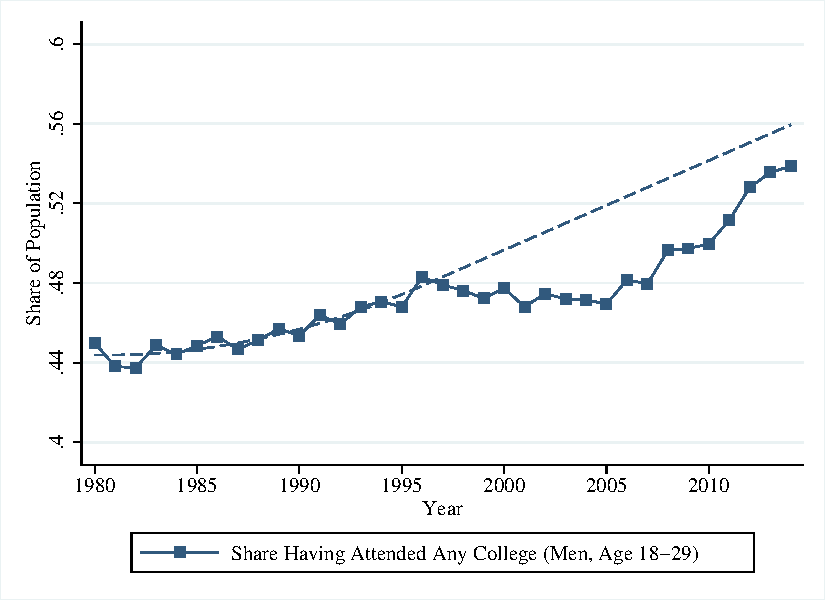
\includegraphics[scale=0.625]{output/fig1_educ_m_18_29.pdf} & \ \ & 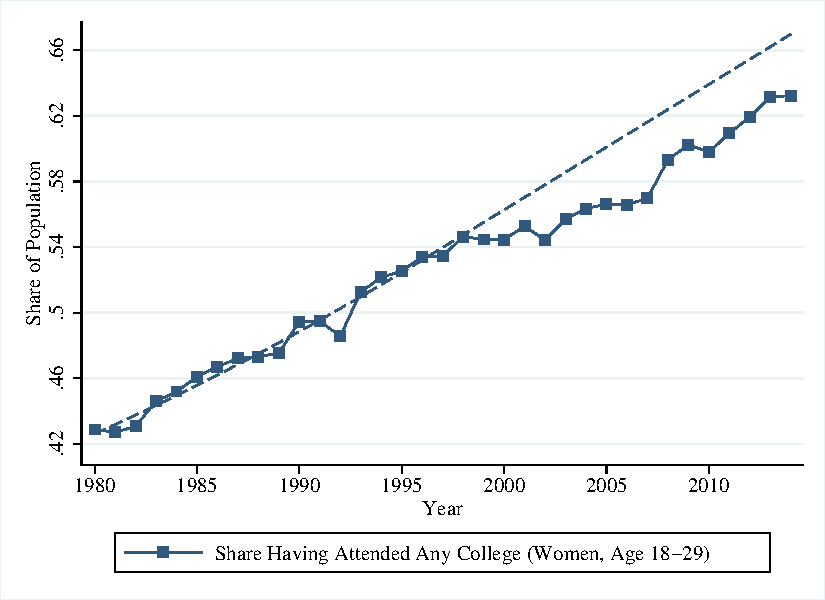
\includegraphics[scale=0.625]{output/fig1_educ_f_18_29.pdf} \\
\end{tabular}
\caption{\underline{Notes:} This figure reports trends in the share of men and women (age 18-29) who have attended at least one year of college.  This series is constructed from the Current Population Survey (CPS) using CPS survey weights.  The dashed line is the predicted college attendance rates based on a quadratic trend that is fit to the 1980-1996 period.}
\begin{tabular}{ccc}
\ & \ & \ \\
\ & \ & \ \\
\ & \ & \ \\
\ & \ & \ \\
\ & \ & \ \\
\multicolumn{3}{c}{Figure 2: Fraction to Have Ever Attended College by Age 25} \\
\multicolumn{3}{c}{By Year of Birth for Men and Women Born Between 1960 and 1989} \\
\ & \ & \ \\
Panel A: Men & \ \ & Panel B: Women \\
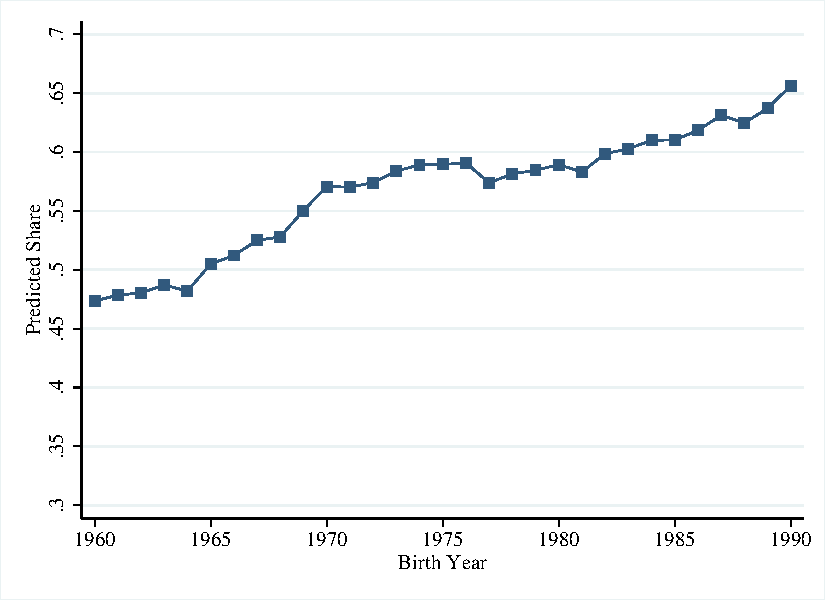
\includegraphics[scale=0.625]{output/fig1_educ_cohort_m.pdf} & \ \ & 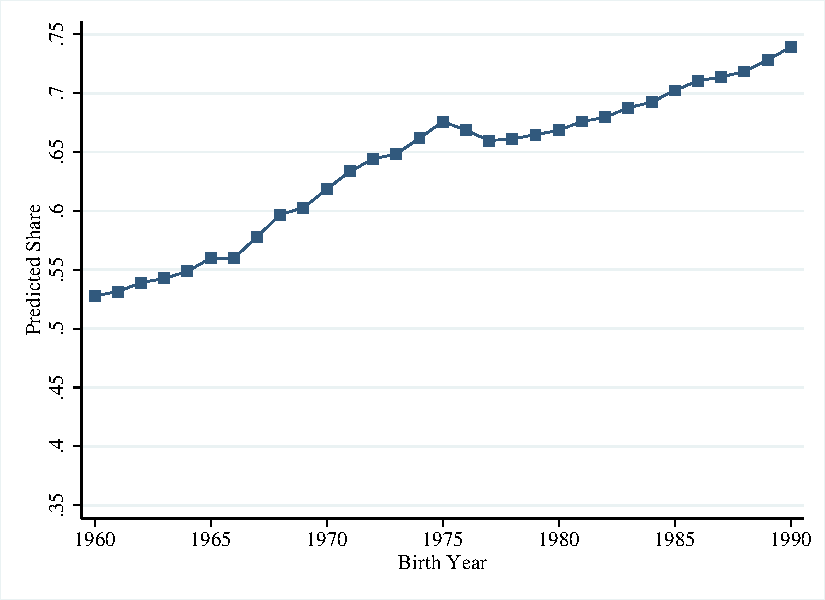
\includegraphics[scale=0.625]{output/fig1_educ_cohort_f.pdf} \\
\end{tabular}
\caption{\underline{Notes:} This figure reports estimated birth year (birth cohort) fixed effects in education for all men and women born between 1960 and 1990 (inclusive). The sample is all individuals between the ages of 25 and 54 (based on age in survey year), pooling CPS data sets between 1994 and 2014.  The birth year fixed effects are recovered from an estimated model that regresses an indicator for whether individual has attended any college on a fourth-degree polynomial in age, birth year fixed effects, and normalized year fixed effects (setting the first and last year fixed effect equal to 0 and the sum of remaining year fixed effects equal to 0). The figures reported fitted values at age 25 using CPS survey weights. The sample is restricted to native-born men and women.}
\end{table}





\clearpage 

\begin{figure}
\begin{center}
Figure 3: Share Any College Attendance for Individuals Born Between 1965 and 1987, by MSA House Price Growth \\
\ \\
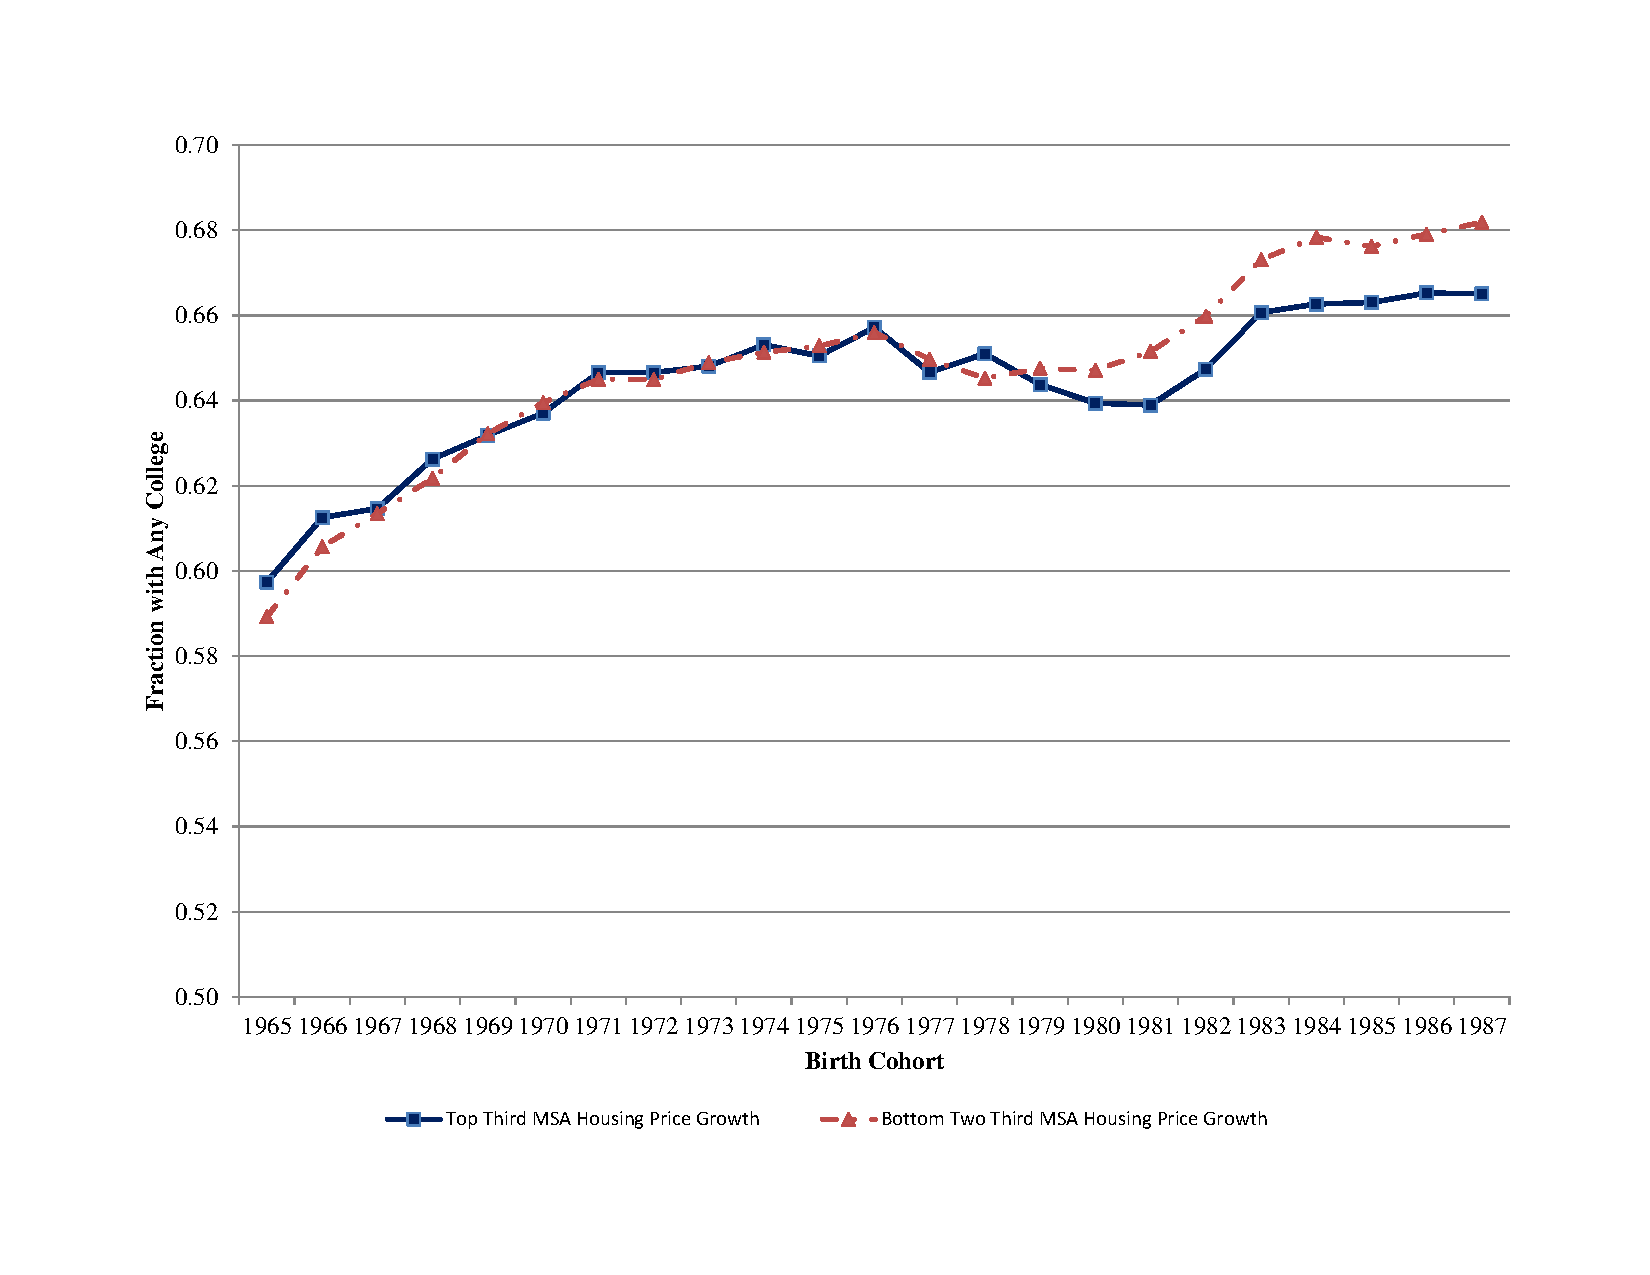
\includegraphics[scale=0.35]{output/fig3_boom_nonboom.pdf} \\
\end{center}
\underline{Notes:} This figure reports education attainment by birth cohort for all men and women born between 1965 and 1987.  The data come from the 1990 Census, the 2000 Census, and the 2005-2013 American Community Survey (ACS). The sample is restricted to all men and women between ages 25 and 54 in the survey year.  The two lines are sub-samples of metropolitan areas based on whether or not the metropolitan was in the top tercile of distribution of house price changes between 2000 and 2006. We use FHFA house price data to compute MSA level house price changes. The data use Census/ACS survey weights.
\ \\
\ \\
\ \\
\begin{center}
Figure 4: Home Prices, Construction/FIRE Employment, Housing Permits, and Housing Transactions in the U.S., 1980-2012 \\
\ \\
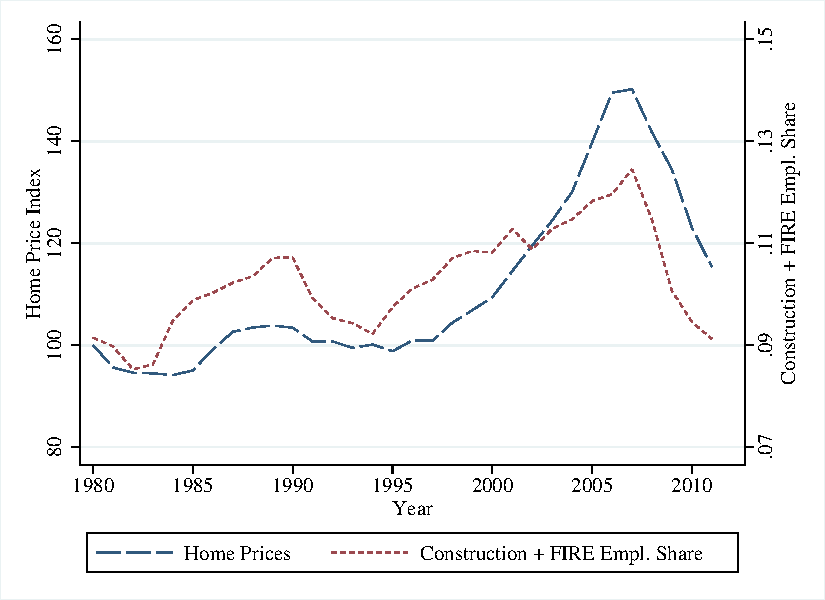
\includegraphics[scale=0.55]{output/fig4a.pdf} \ \ \
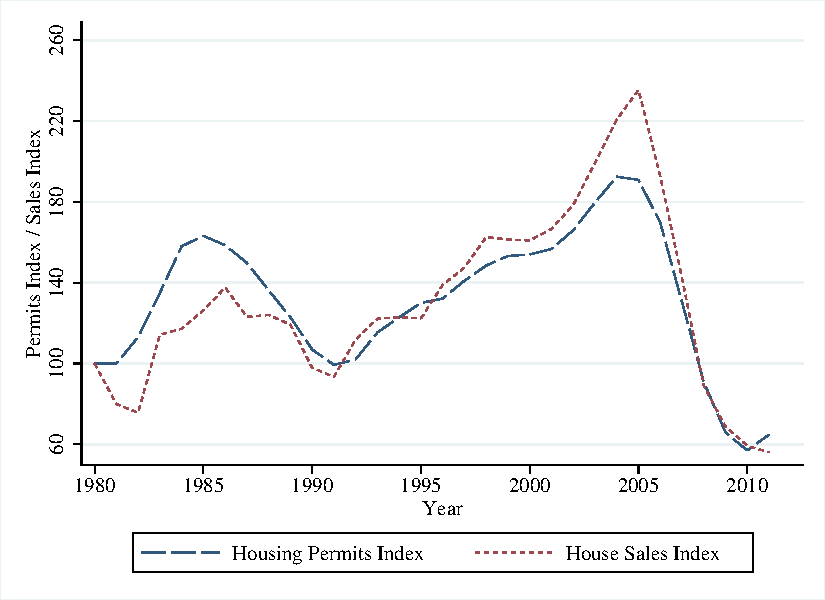
\includegraphics[scale=0.55]{output/fig4b.pdf} \\
\end{center}
\underline{Notes:} These figures report trends in the FHFA National Home Price Index (1980 = 100), trends in the share of population employed in construction and FIRE (finance, insurance, and real estate), trends in the Census Housing Permits Index (1980 = 100), and trends in total new home sales from the Survey of Construction (1980 = 100).  The FHFA series is a weighted, repeat-sales index
that measures average changes in house prices across 363 metropolitan areas.  The Census series is a building permits survey that estimates the number of new housing units (as authorized by building permits). The Survey of Construction series measures new house sales of single-family homes, whether or not building new homes in those areas requires a building permit.  The population employment shares are calculated from Current Population Survey and are based on all prime-age men and women (age 18-55).
\end{figure}


\clearpage

\begin{table}
\centering
\begin{tabular}{ccc}
\multicolumn{3}{c}{Figure 5: An Economic Model of College Attendance} \\
\ & \ & \ \\
Panel A:  College Attendance Decisions by Ability & \ \ & Panel B: Increase in $Y^0_t$ From Housing Boom \\
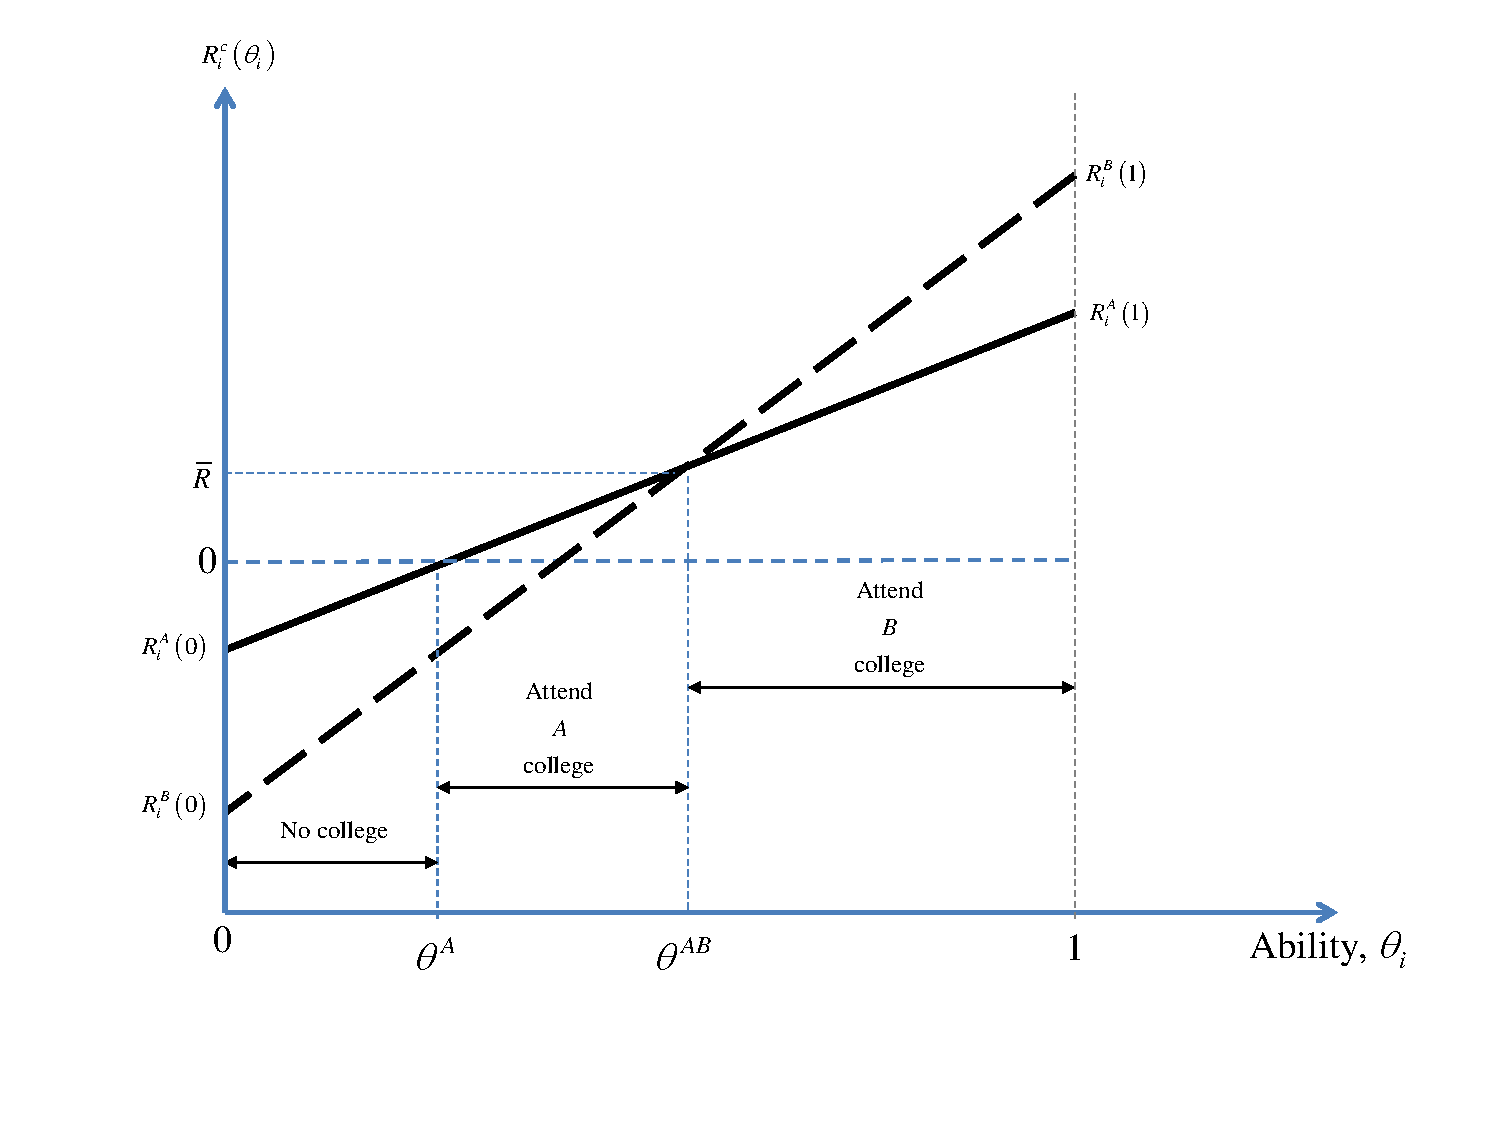
\includegraphics[scale=0.42]{output/fig5_graph_ed_model1.pdf} & \ \ & 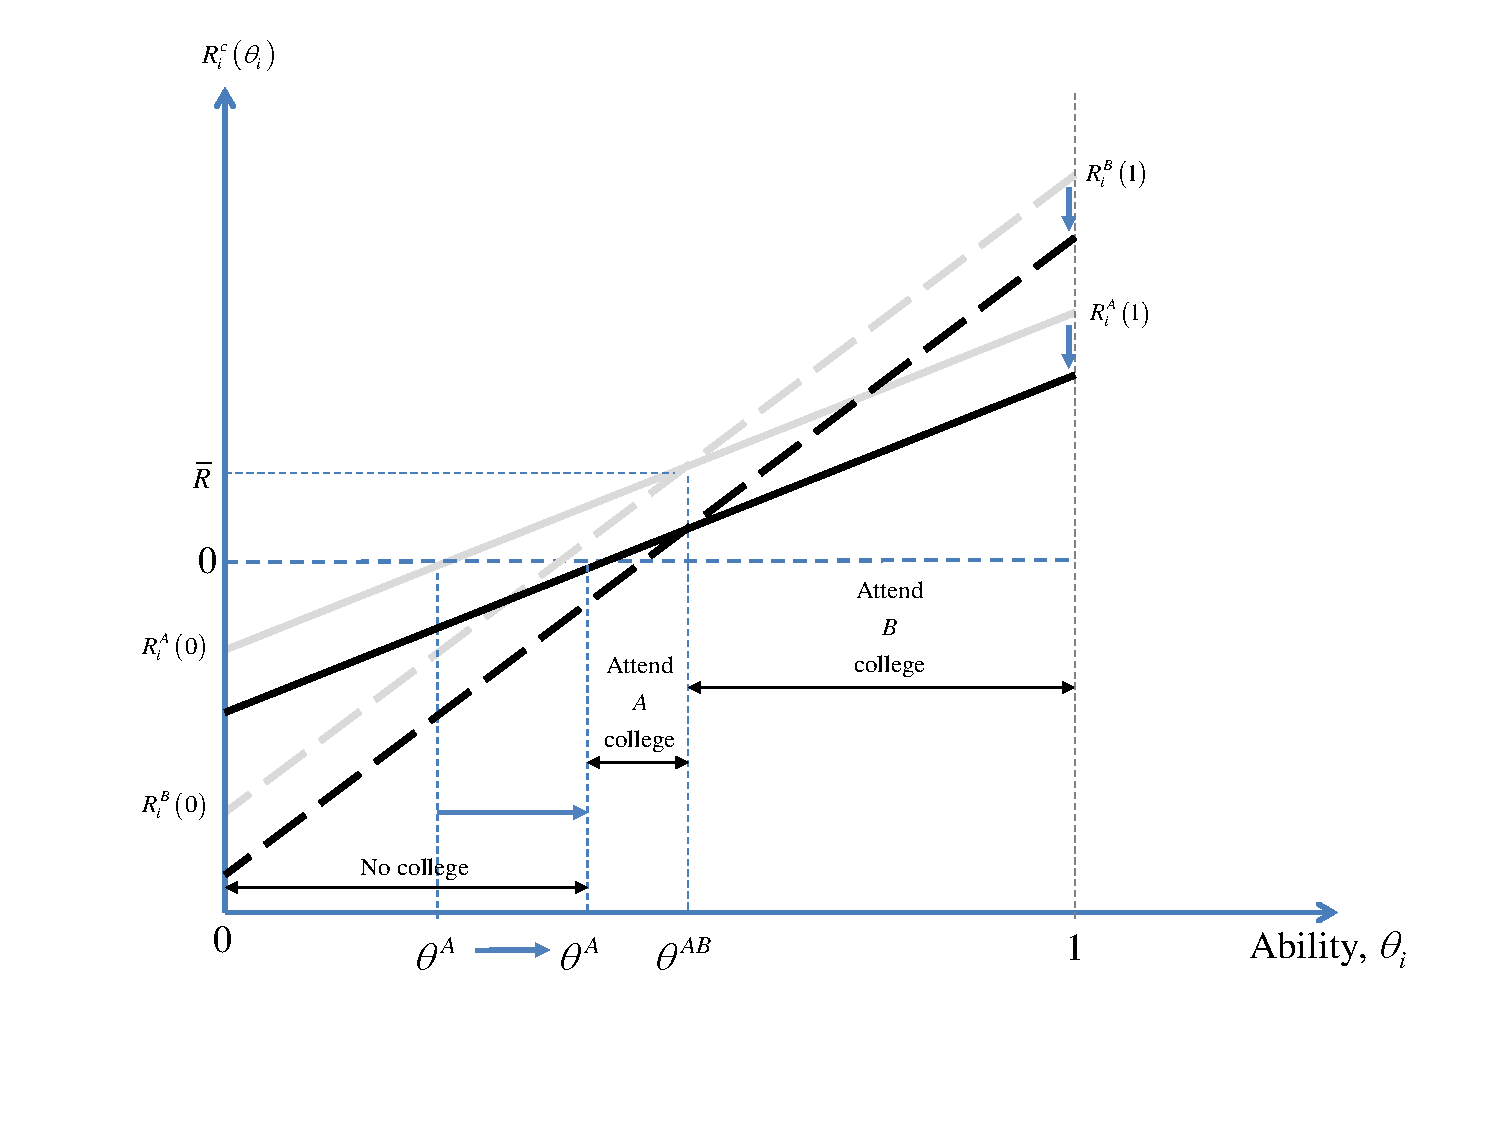
\includegraphics[scale=0.42]{output/fig5_graph_ed_model2.pdf} \\
\end{tabular}
\caption{\underline{Notes:} This figure shows the equilibrium college attendance decisions for individuals as a function of their underlying ability. The equilibrium shows individuals making choices of whether to attend college (and, if so, whether to attend type-$A$ ``Associate's'' college or type-$B$ ``Bachelors'' college). In the equilibrium, individuals sort based on comparative advantage, with low-ability individuals not attending college, middle-ability individuals attending type-$A$ college, and high-ability individuals attending type-$B$ college.  In Panel B, there is a positive housing demand shock (housing boom), which raises income of all non-college-educated individuals by the same amount. In the new equilibrium, there is a reduction in share of population attending type-$A$ college but no change in share attending type-$B$ college.}
\end{table}


\clearpage

\begin{figure}[!tp]
\begin{center}
Figure 6: Correlation Between Changes in Housing Permits and Home Prices, 2000-2006
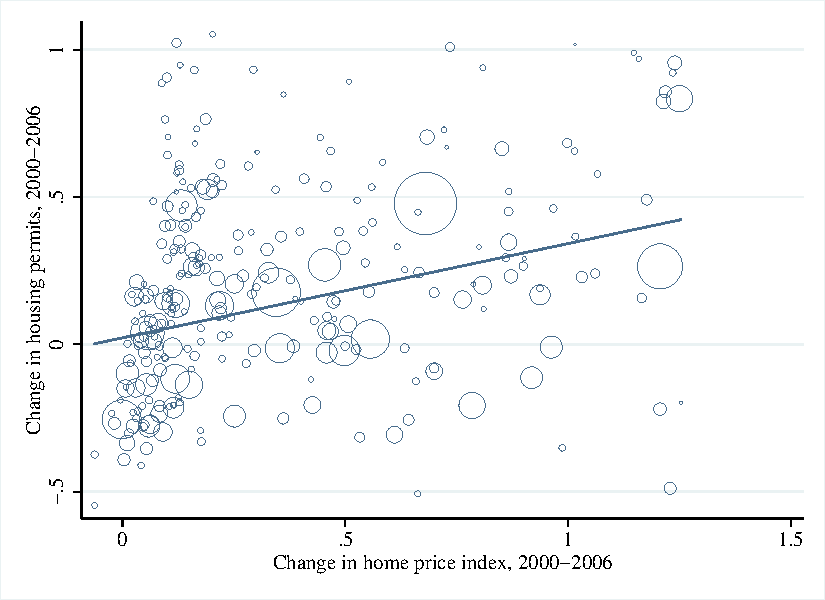
\includegraphics[scale=0.65]{output/fig6_scatter_dp_dq.pdf} \\
\end{center}
\underline{Notes:} This figure shows correlation between changes in home price index and housing permit index.  The regression line is weighted regression using 18-55 adult population as weights, and the sample is the baseline sample of 275 MSAs used in main regression tables.
\end{figure}
\ \\ 
\ \\ 
\begin{figure}[!h]
\begin{center}
Figure 7: Trends in Housing Demand Over Time and Across Metropolitan Areas \\
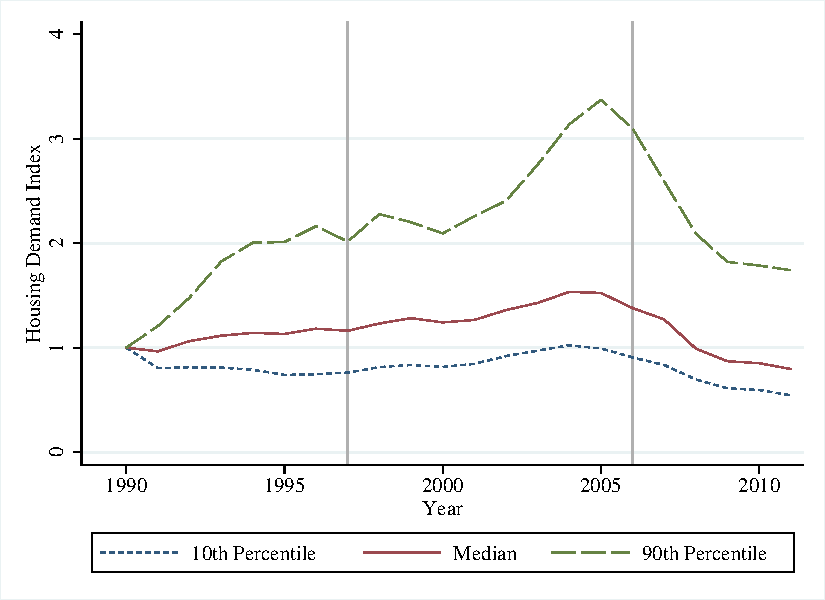
\includegraphics[scale=0.75]{output/fig7_demand_pctiles.pdf} \\
\end{center} 
\underline{Notes:} This figure reports trends in our constructed housing demand index (which is the log sum of the prices and permits indexes) at the 10th percentile, median, and 90th percentile, normalized to 1980 values within each percentile.
\end{figure}


\clearpage 


\begin{table}
\centering
\begin{tabular}{ccc}
\multicolumn{3}{c}{Figure 8: Variation in Structural Break Across Cities} \\
\ & \ & \ \\
Citis without Structural Break & \ \ \ \ & Cities with Structural Break \\
\ & \ & \ \\
Pittsburgh, PA [No Break] & \ \ & Portland, OR [Small Break] \\
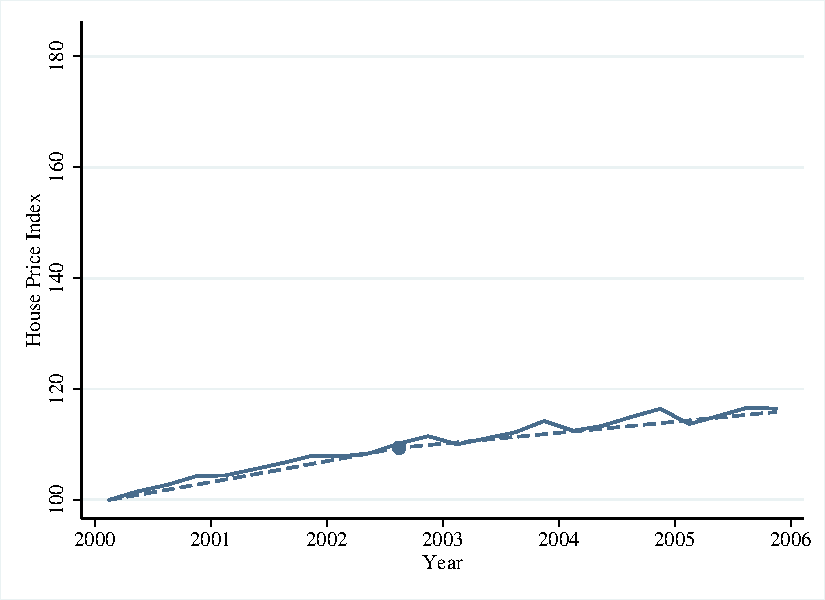
\includegraphics[scale=0.588]{output/fig8_fhfa_pair1.pdf} & \ \ & 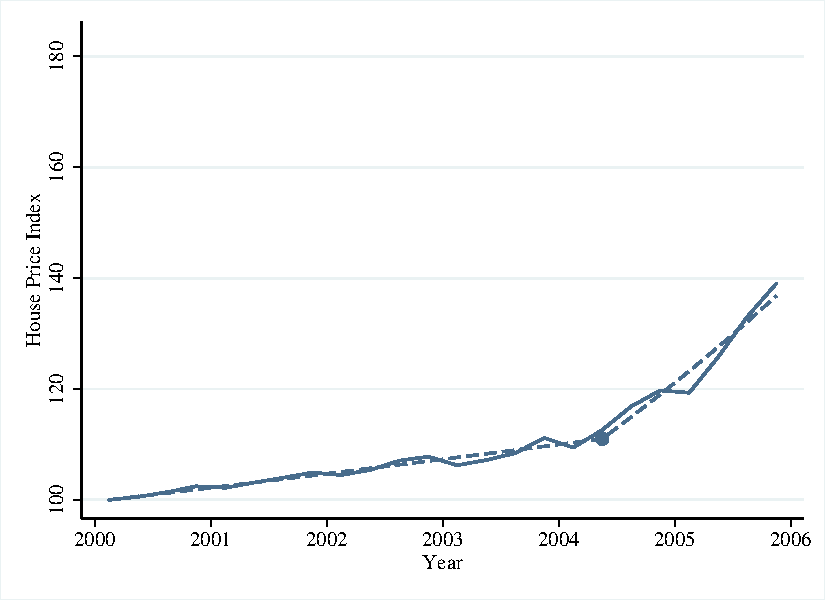
\includegraphics[scale=0.588]{output/fig8_fhfa_pair4.pdf} \\
\ & \ & \ \\
Chicago, IL [No Break] & \ \ & Tucson, AZ [Medium Break] \\
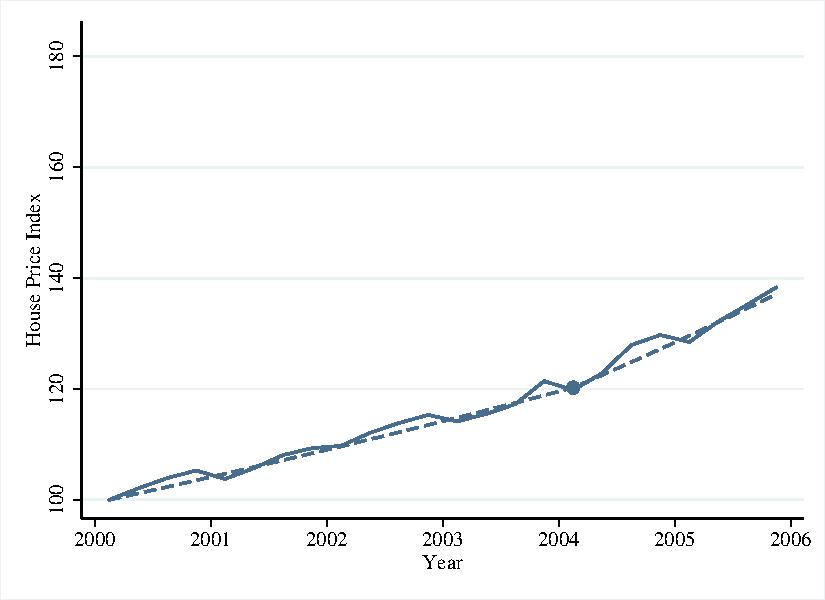
\includegraphics[scale=0.588]{output/fig8_fhfa_pair2.pdf} & \ \ & 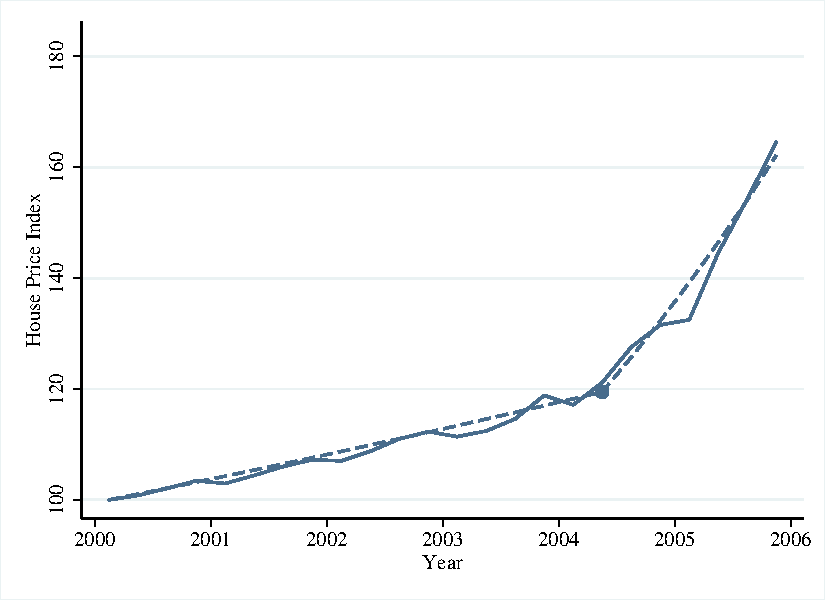
\includegraphics[scale=0.588]{output/fig8_fhfa_pair5.pdf} \\
\ & \ & \ \\
New Haven, CT [No Break] & \ \ & Naples, FL [Large Break] \\
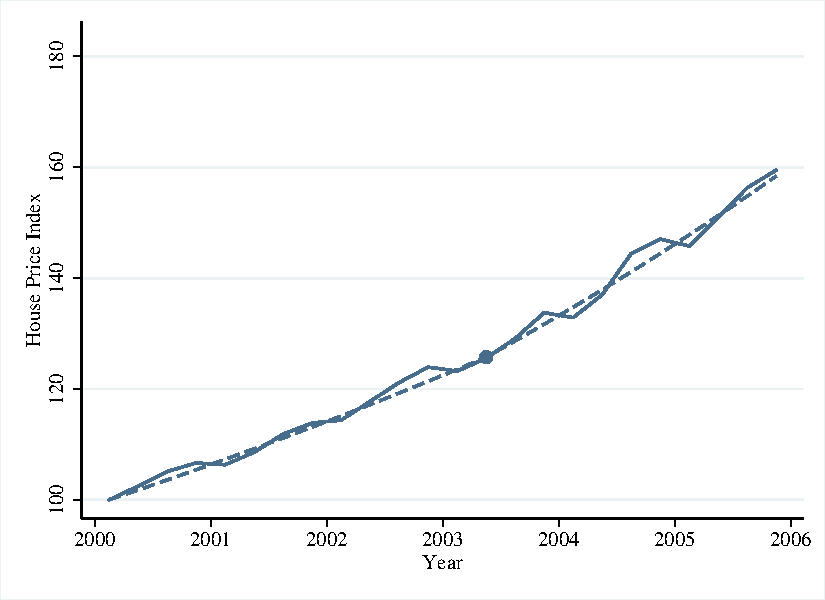
\includegraphics[scale=0.588]{output/fig8_fhfa_pair3.pdf} & \ \ & 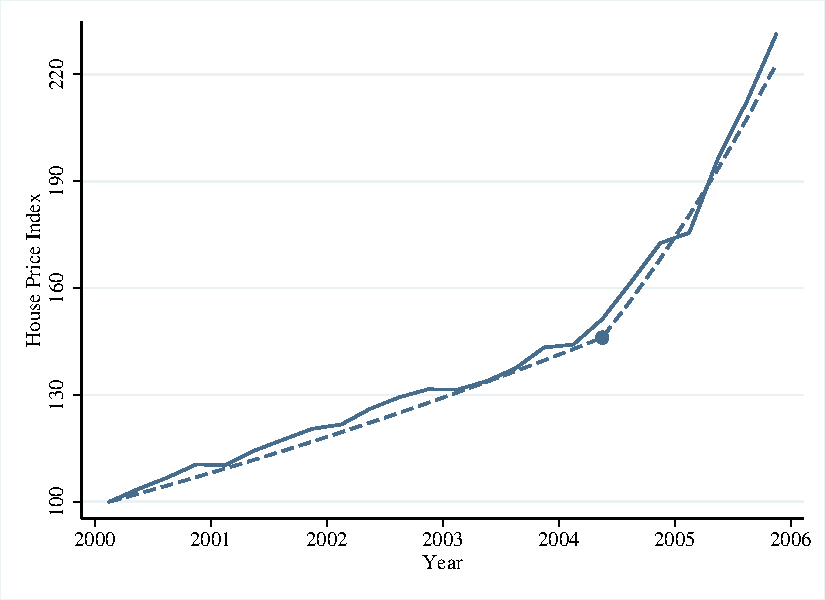
\includegraphics[scale=0.588]{output/fig8_fhfa_pair6.pdf} \\
\end{tabular}
\end{table}
\begin{figure}[!b]
\underline{Notes:} This figure shows graphs of quarterly house price data for six MSAs.  The house price index for each city is normalized so that Q1, 2000 = 100.  The solid lines report the house price series, while the dashed lines reports the structural break estimates, with a solid dot indicating the estimated quarter of the structural break. The MSAs in first column have small estimated structural breaks, and the MSAs in the second column have relatively larger estimated structural breaks.  The rows group MSAs based on overall house price growth up until the estimated structural break.
\end{figure}


\clearpage

\begin{figure}
\begin{center}
Figure 9: First Stage Relationship Between Instrument and Change in Housing Demand \\ 
\ \\
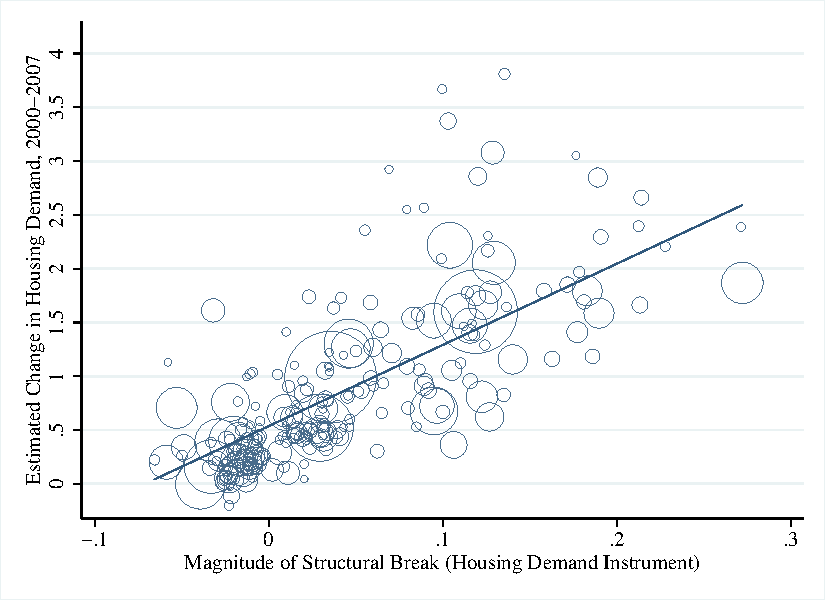
\includegraphics[scale=0.65]{output/fig9_fhfaB.pdf} \\
\end{center}
\underline{Notes:} This figure shows the correlation across cities between the magnitude of structural break and the estimated housing demand change across 2000-2006.  The Magnitude of Structural Break variable corresponds to the (annualized) coefficient from the city-specific structural break regression.  The higher the value of the instrument, the larger the estimated structural break.
\ \\
\ \\
\ \\
\begin{center}
Figure 10: House Price Growth, 2006-2012 versus 2000-2006 \\
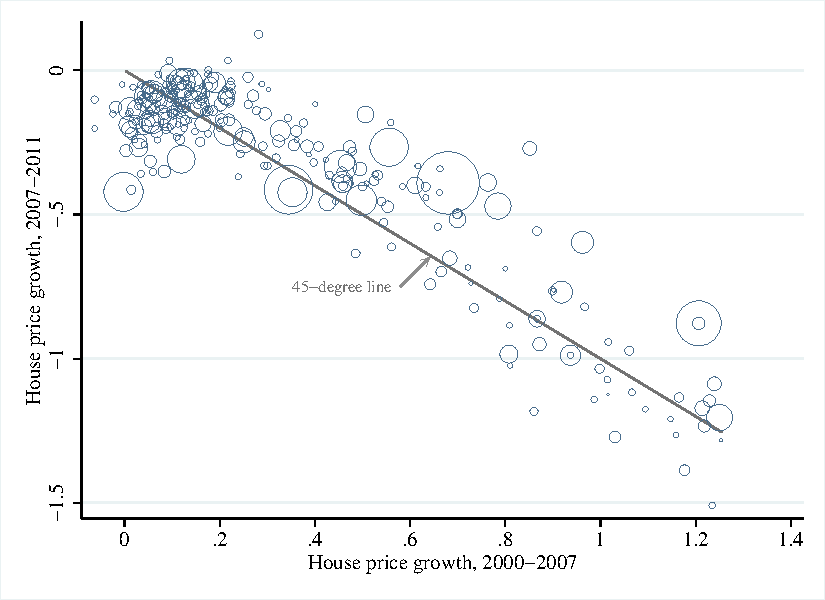
\includegraphics[scale=0.7]{output/fig10_scatter.pdf} \\
\end{center}
\underline{Notes:} This figure shows the correlation between the change in house prices in 2000-2006 and the change in house prices in 2006-2012 for the 275 MSAs in our baseline sample.  The dotted line is a 45-degree line (i.e., slope of -1).  
\end{figure}


\clearpage

\begin{table}[!t]
\centering
\begin{tabular}{cc}
\multicolumn{2}{c}{Figure 11: Lack of Correlation Between Structural Break Instrument and ...} \\
\ & \ \\
Lagged Change in House Price Index, 1990-1995 & Lagged House Price Index, 1990 \\
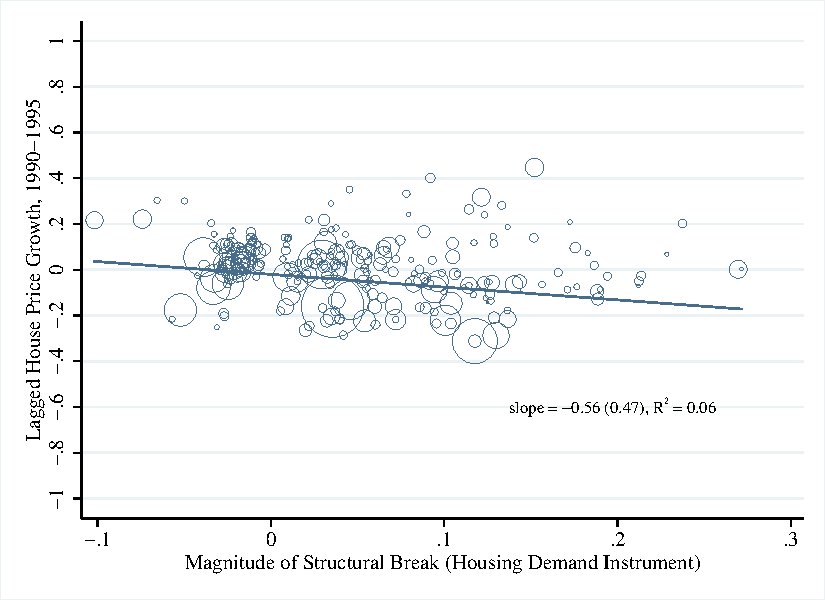
\includegraphics[scale=0.45]{output/fig11_corr_lagged_hp.pdf} & 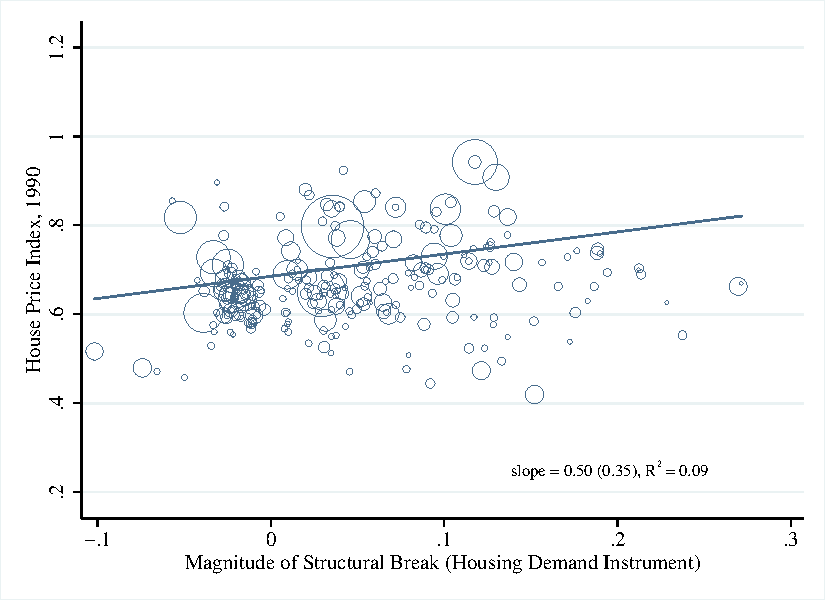
\includegraphics[scale=0.45]{output/fig11_corr_hpi1990.pdf} \\
\ & \ \\
Change in Two-Year Enrollment Per Capita, 1990-1995 & Two-Year Enrollment Per Capita, 1990 \\
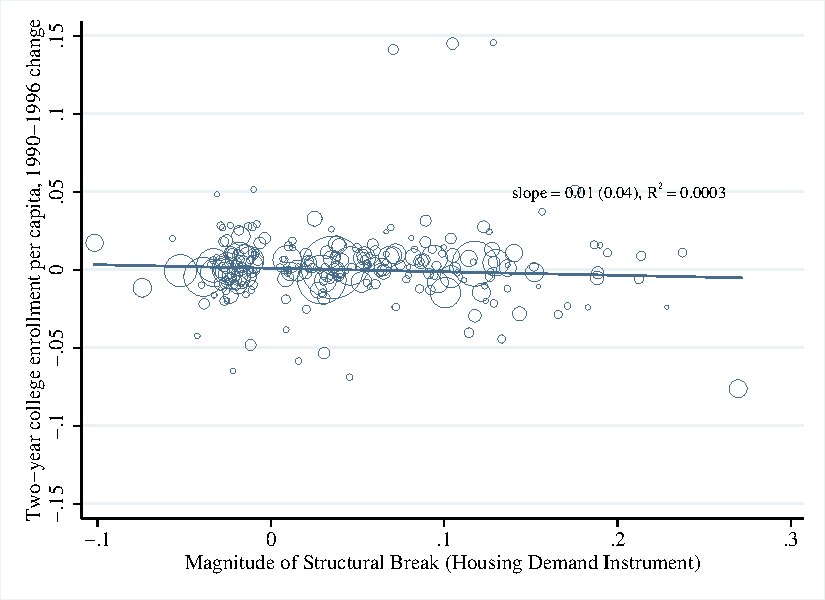
\includegraphics[scale=0.45]{output/fig11_corr_diff_a2.pdf} & 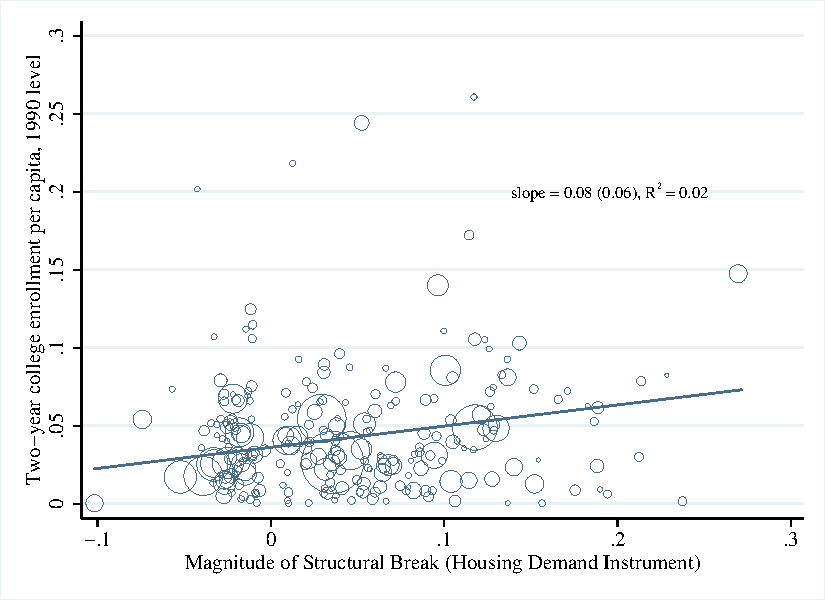
\includegraphics[scale=0.45]{output/fig11_corr_init_a2.pdf} \\
\ & \ \\
Change in Four-Year Enrollment Per Capita, 1990-1995 & Four-Year Enrollment Per Capita, 1990 \\
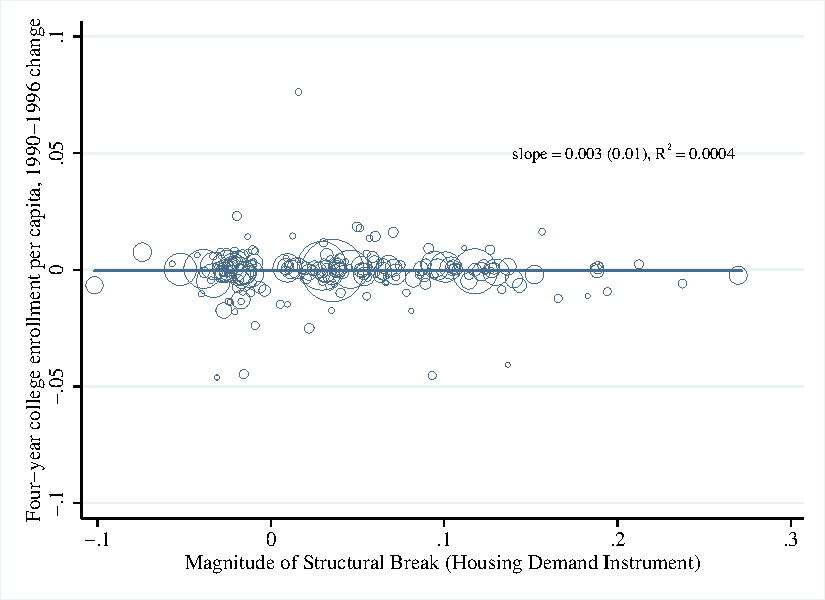
\includegraphics[scale=0.45]{output/fig11_corr_diff_a34.pdf} & 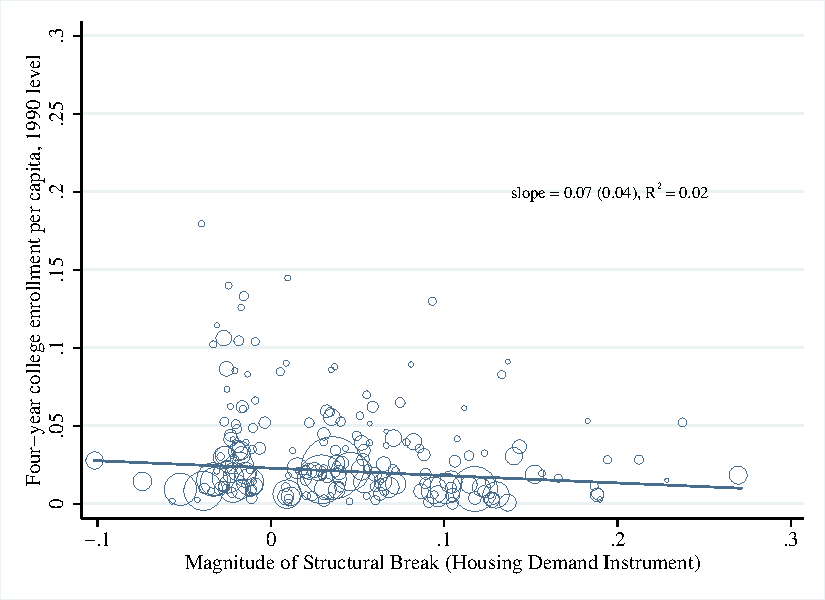
\includegraphics[scale=0.45]{output/fig11_corr_init_a34.pdf} \\
\ & \ \\
Employment Rate, 1990 & Average Wages, 1990 \\
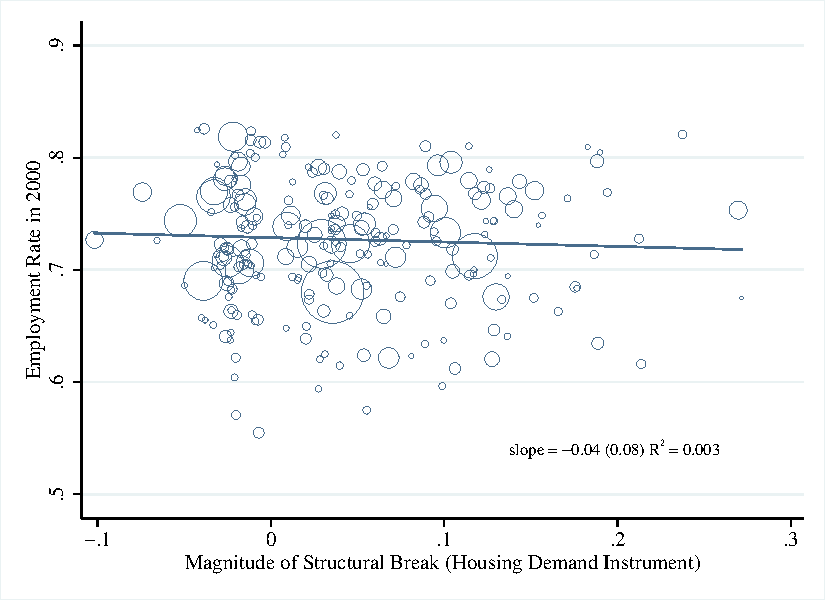
\includegraphics[scale=0.45]{output/fig11_corr_init_emp.pdf} & 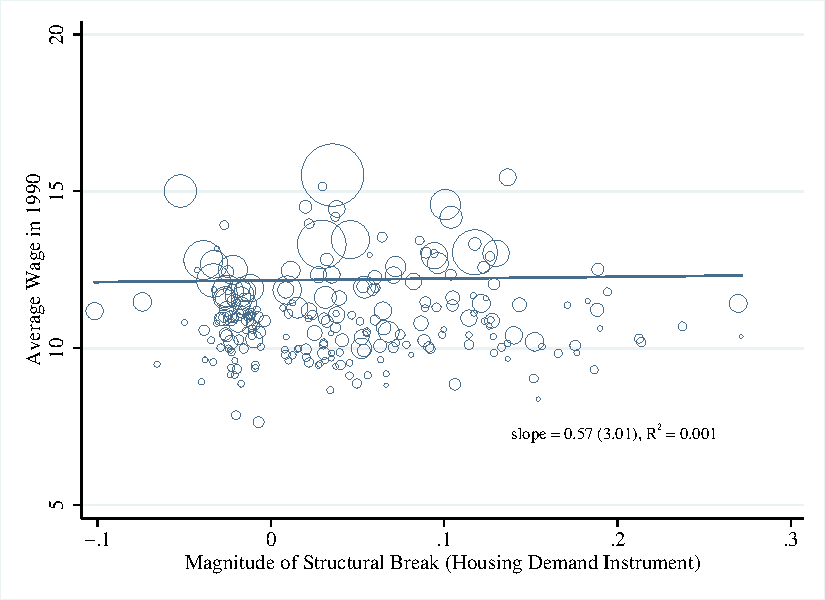
\includegraphics[scale=0.45]{output/fig11_corr_init_wage.pdf} \\
\ & \ \\
\end{tabular}
\caption{\underline{Notes:} This figure reports the correlation between
  the structural break instrument used in the IV specifications and lagged levels and changes in house prices,
  emlpoyment rate, wages, and two-year and four-year college enrollment (per capita). }
\end{table}


\clearpage


\begin{table}
\centering
\begin{tabular}{cc}
\multicolumn{2}{c}{Figure 12: Significant Correlation Between Structural Break Instrument and ...} \\
\ & \ \\
Growth in Price-Rent Ratio & Change in ``Out-of-Town'' Buyers Share \\
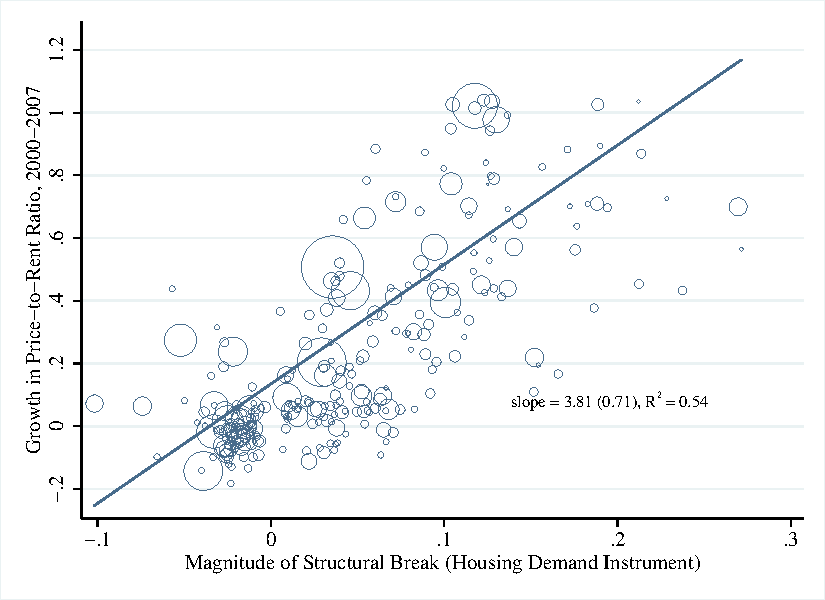
\includegraphics[scale=0.55]{output/fig12_price_rent_full.pdf} & 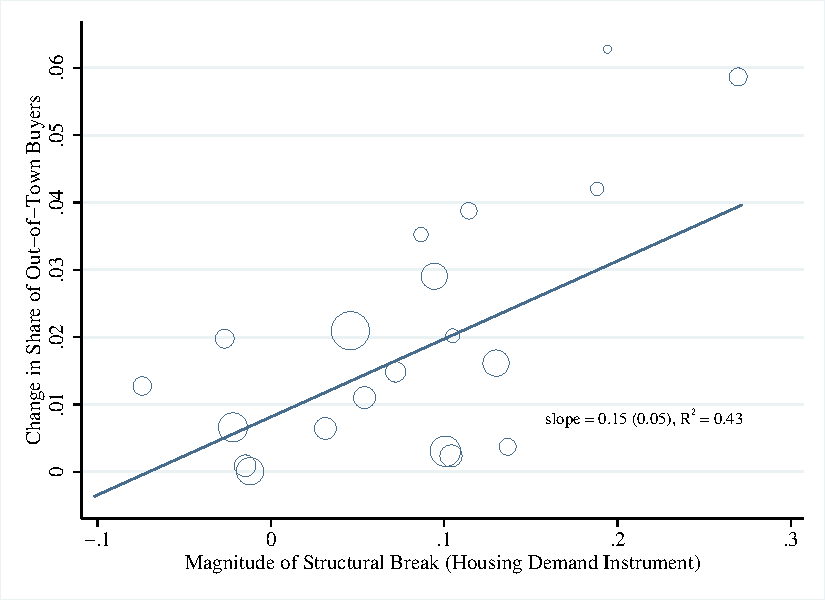
\includegraphics[scale=0.55]{output/fig12_corr_mayer.pdf} \\
\ & \ \\
Structural Break in Volume & Structural Break in Price+Volume \\
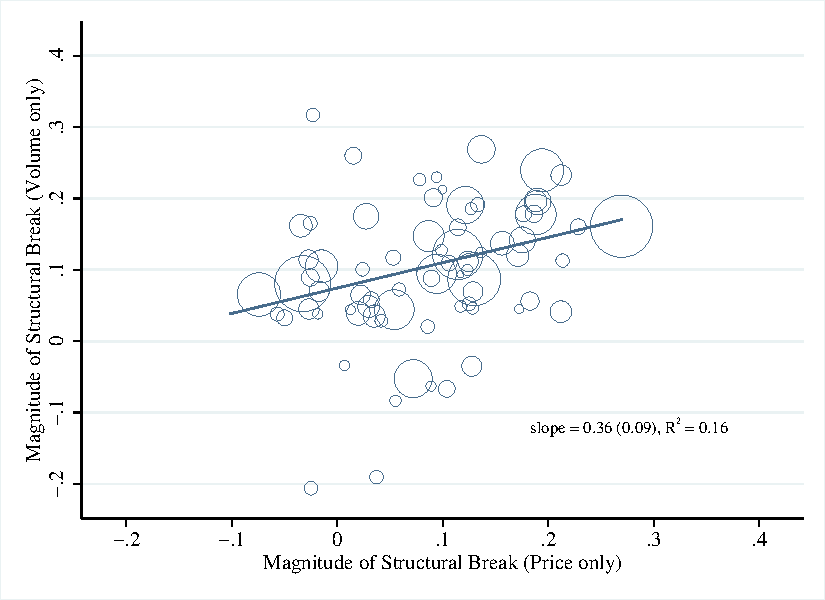
\includegraphics[scale=0.55]{output/fig12_corr_vol.pdf} & 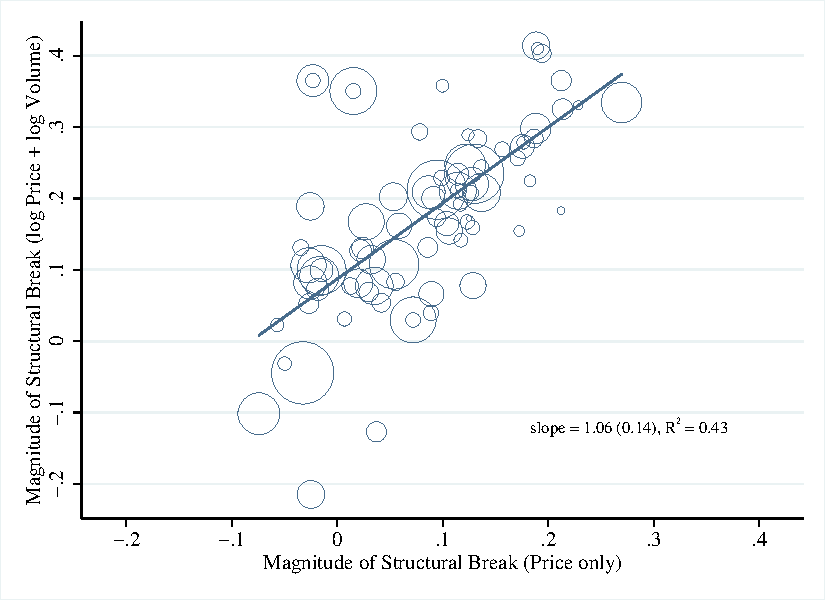
\includegraphics[scale=0.55]{output/fig12_corr_vol2.pdf} \\
\ & \ \\
\end{tabular}
\caption{\underline{Notes:} The first row in this figure reports the correlation between
the structural break instrument used in the IV specifications and
the growth in the price-rent ratio and the change in the share of ``out-of-town'' buyers, which can be interpreted as proxies for speculation.
See text for details of the price-rent ratio calculation and the source of the ``out of town'' buyer share. The second row of this figure reports correlation between estimated magnitude of structural break in housing volume (from DataQuick) and house prices (from FHFA data), as well as correlation between strutural break in prices and estimated structural break in Price and Volume combined. All structural breaks are estimated using log-linear models, so that Price+Volume estimates break in log(Price*Volume).}
\end{table}


\clearpage

\begin{figure}[!tp]
\begin{center}
Figure 13: Event Study Analaysis of Per Capita College Attendance \\
\ \\
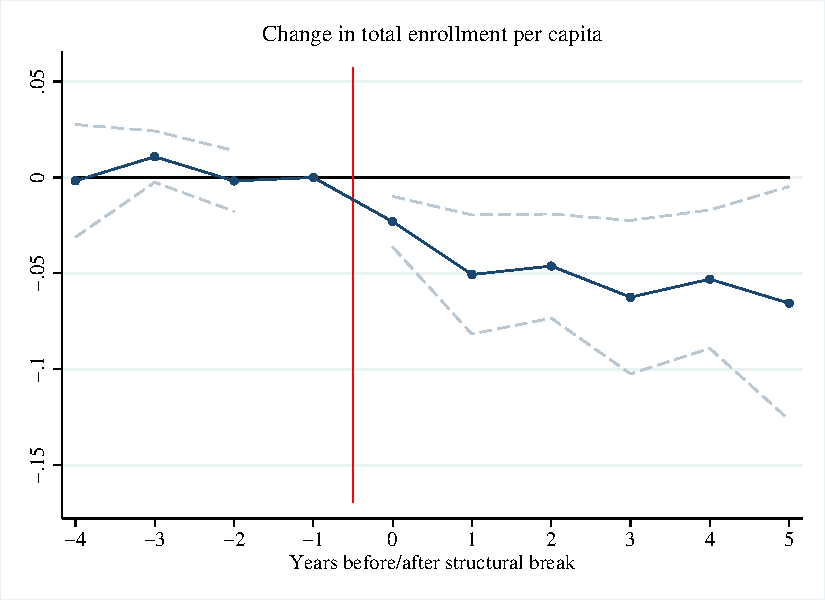
\includegraphics[scale=0.85]{output/fig13_ipeds_evt_study_assoc_enrollment.pdf} \\
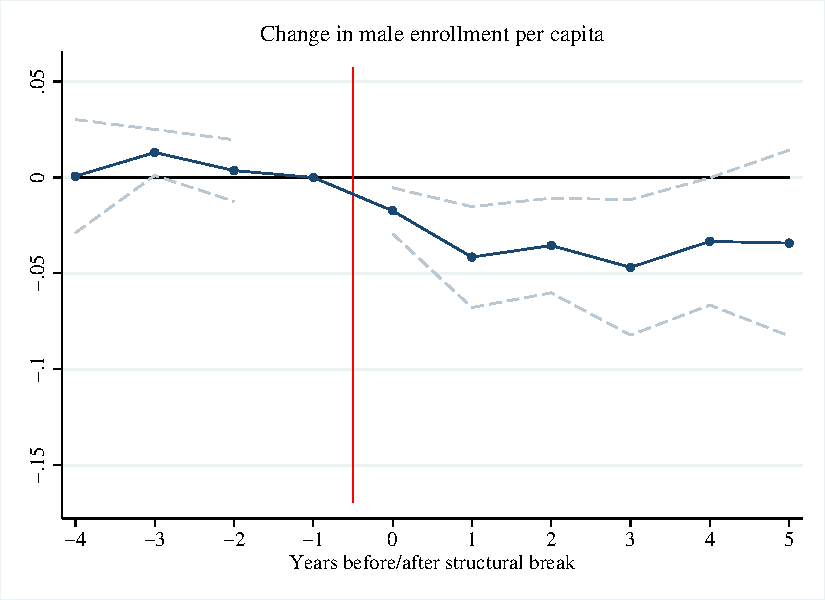
\includegraphics[scale=0.55]{output/fig13_ipeds_evt_study_assoc_men.pdf} \ \ \
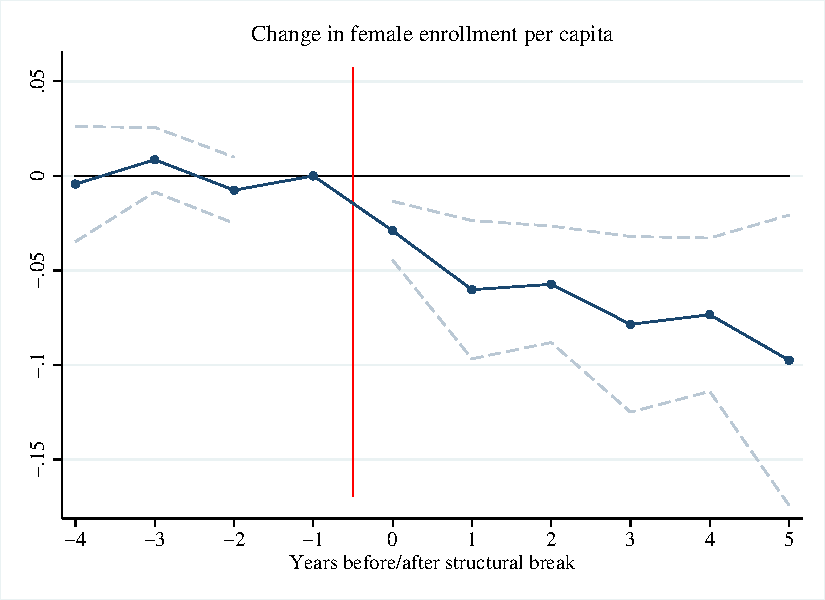
\includegraphics[scale=0.55]{output/fig13_ipeds_evt_study_assoc_women.pdf} \\
\end{center}
\underline{Notes:} This figure reports esetimates of event study regressions, which include indicator variables for each year before and after year of estimated structural break, which the indicator scaled by the magnitude of the structural break.  The event study regression specification includes year fixed effects and metropolitan area fixed effects and is weighted by the overall population in 1990.  The structural break is allowed to be anywhere between 1995Q1 and 2005Q1.  The college enrollment data come from IPEDS and restrict to two-year colleges and universities.  The population data focuses on 18-25 year olds and are estimated using county-by-age population estimates from the Survey of Epidemiology and End Results (SEER) data set. The sample period in each metropolitan area is restricted to 6 years before and after estimated structural break (if available).  Standard errors are clustered by state.
\end{figure}











\clearpage 

\begin{figure}[!tp]
\begin{center}
Online Appendix Figure OA.1: College Attendance Decisions Following a Housing Boom \\
\ \\
Attendance Decisions Following \emph{Large} Increase in $Y^0_t$ From Housing Boom \\
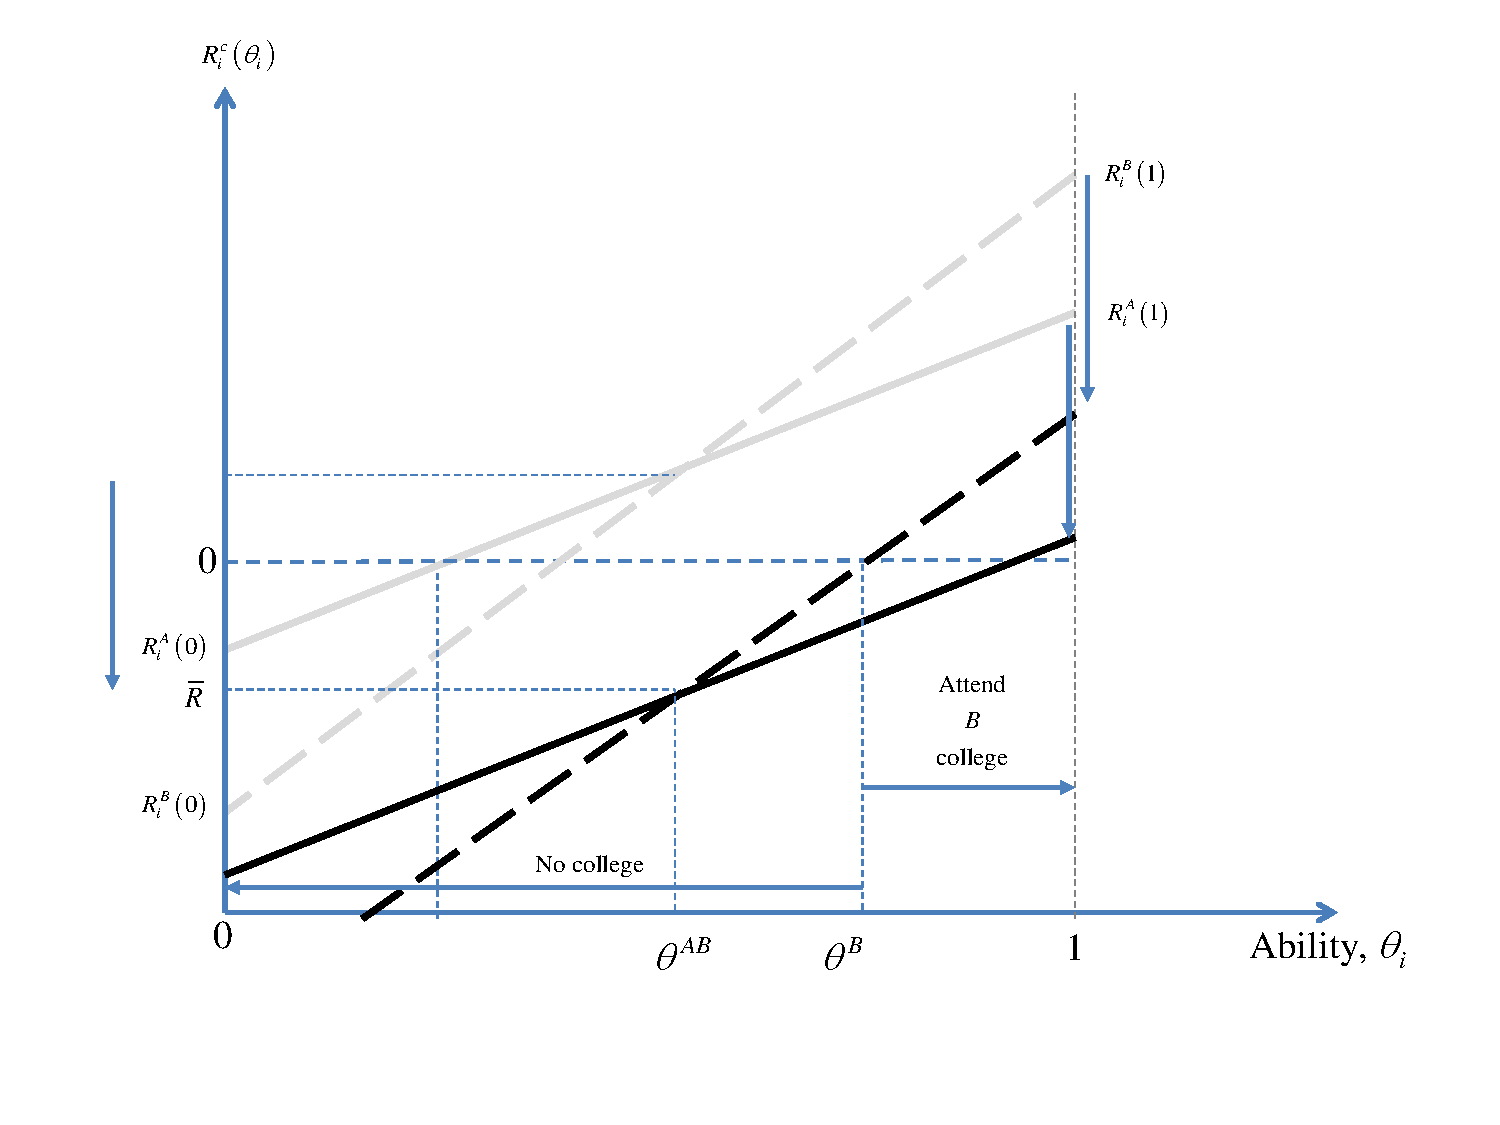
\includegraphics[scale=0.5]{output/fig5_graph_ed_model3.pdf} \\
\end{center}
\underline{Notes:} 
This figure shows college attendance decisions for individuals as a function of underlying ability, extending Figure 6 by showing the consequences of a housing boom.  Only in extreme case of a very large housing boom will the share of individuals attending $H$ college be affected.
\end{figure}


\clearpage


\begin{table}
\centering
\begin{tabular}{ccc}
\multicolumn{3}{c}{Online Appendix Figure OA.2: Randomization tests exploiting timing and magnitude of local housing boom} \\
\ & \ & \ \\
Two-year colleges & \ \ \ \ & Four-year universities \\
\ & \ & \ \\
All adults & \ \ & All adults \\
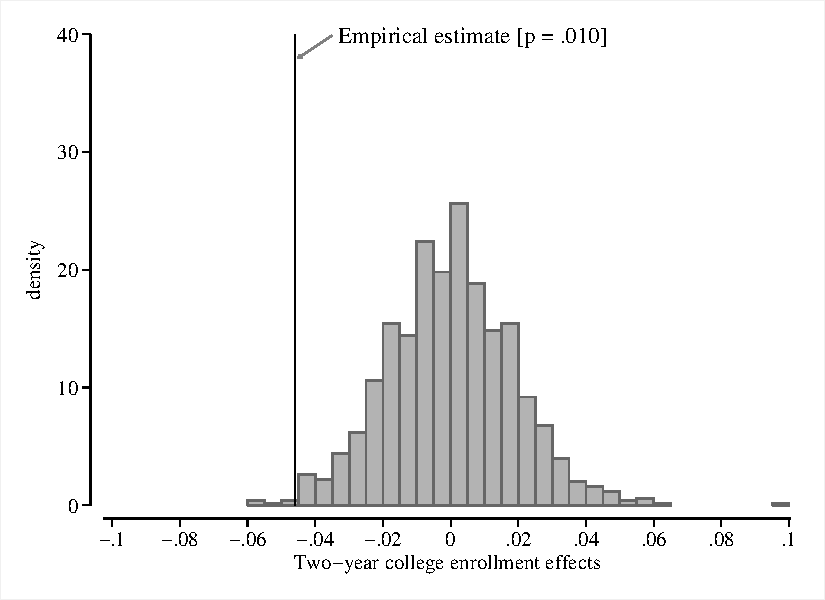
\includegraphics[scale=0.588]{output/permutation/permutation_enrollment_1.pdf} & \ \ & 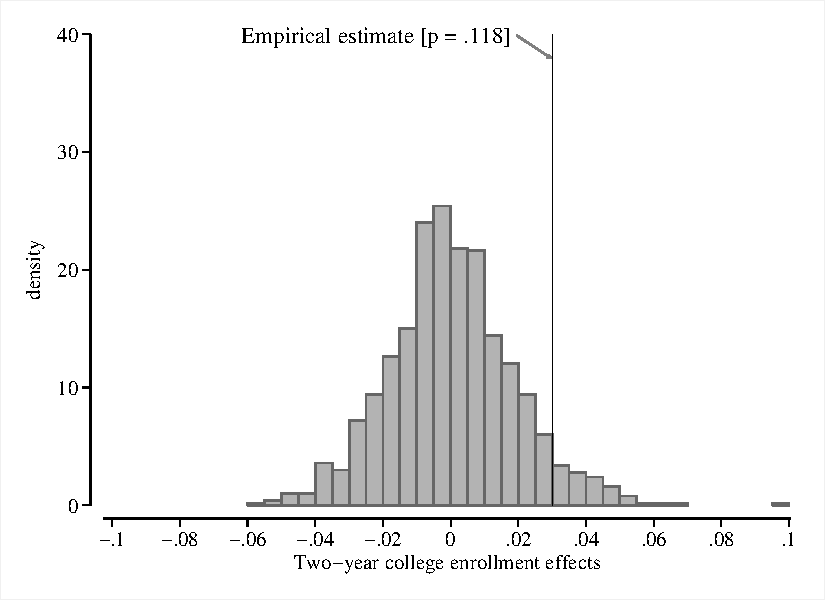
\includegraphics[scale=0.588]{output/permutation/permutation_enrollment_2.pdf} \\
\ & \ & \ \\
Men & \ \ & Men \\
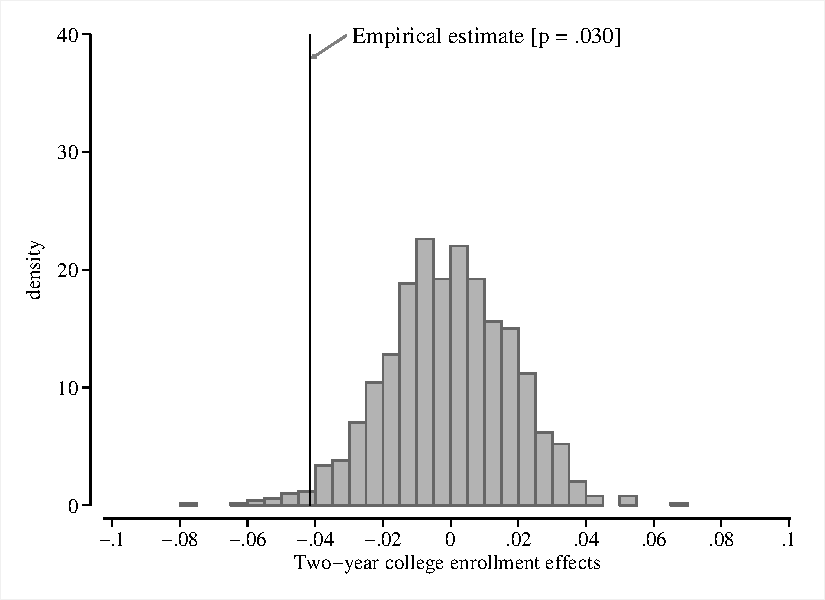
\includegraphics[scale=0.588]{output/permutation/permutation_men_1.pdf} & \ \ & 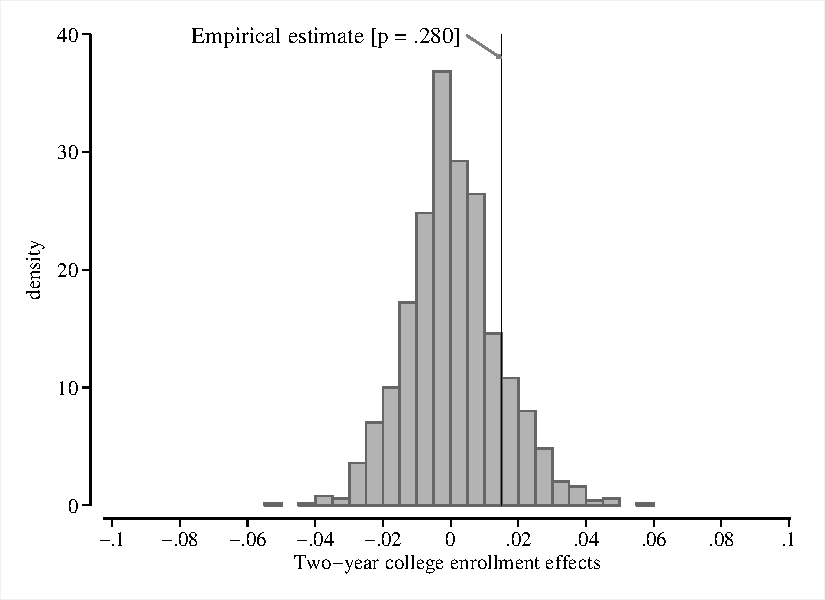
\includegraphics[scale=0.588]{output/permutation/permutation_men_2.pdf} \\
\ & \ & \ \\
Women & \ \ & Women \\
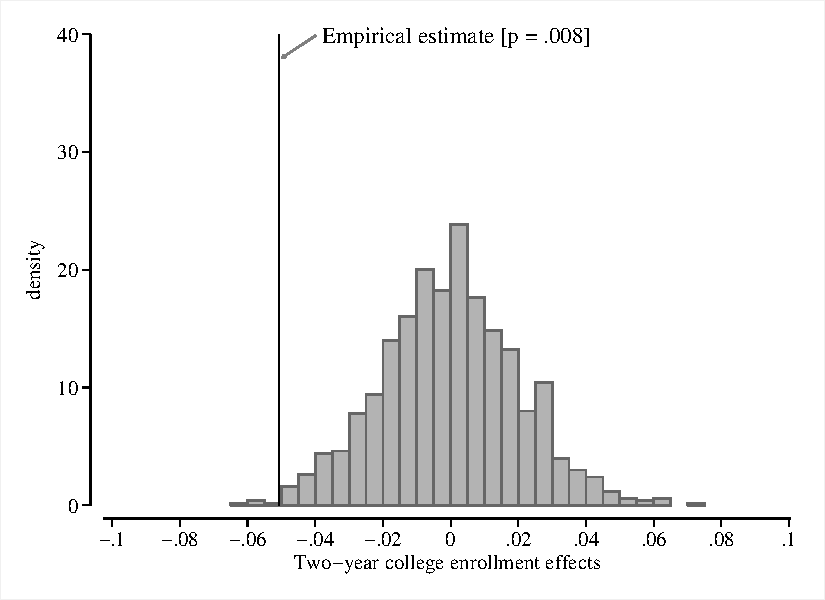
\includegraphics[scale=0.588]{output/permutation/permutation_women_1.pdf} & \ \ & 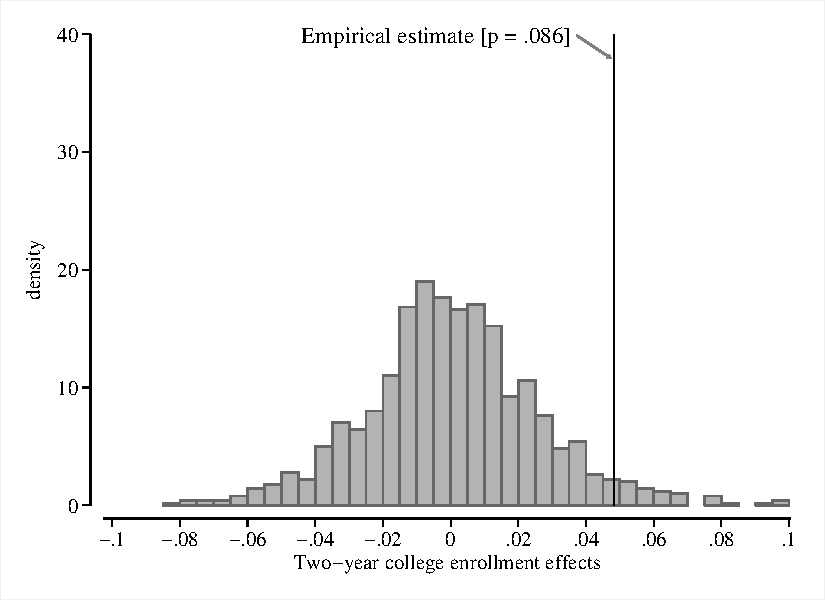
\includegraphics[scale=0.588]{output/permutation/permutation_women_2.pdf} \\
\end{tabular}
\end{table}
\begin{figure}[!p]
\underline{Notes:} This figure shows histograms of distribution of estimated effects of housing boom on two-year and four-year college enrollment per capita for 1,000 permutation samples which permute the magnitude and year of structural break in local house prices across each city. The vertical lines indicate the corresponding estimates from the true data shown in Table 5. 
\end{figure}

\clearpage


\begin{figure}[!tp]
\begin{center}
Online Appendix Figure OA.3: Event Study Analaysis of Employment and Income \\
\ \\
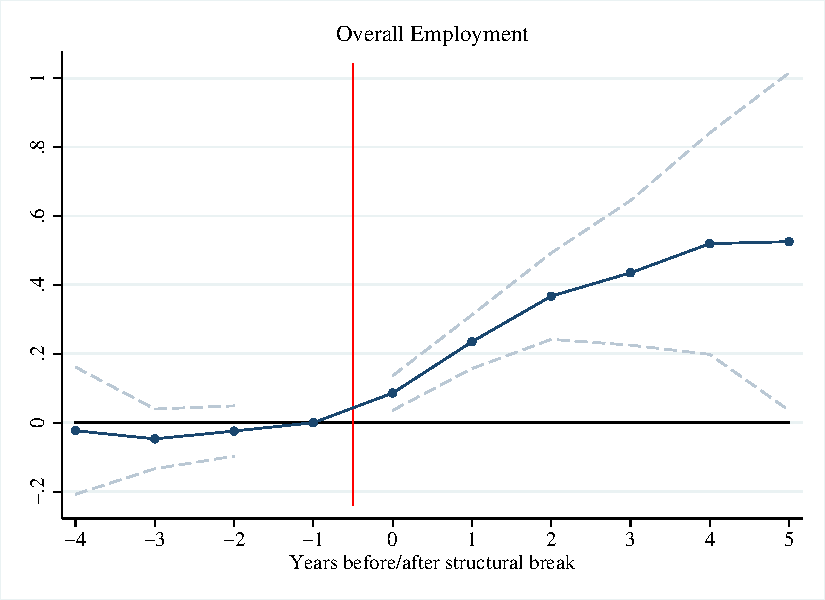
\includegraphics[scale=0.59]{output/cbp_evt_study_emp_.pdf} \ \ \
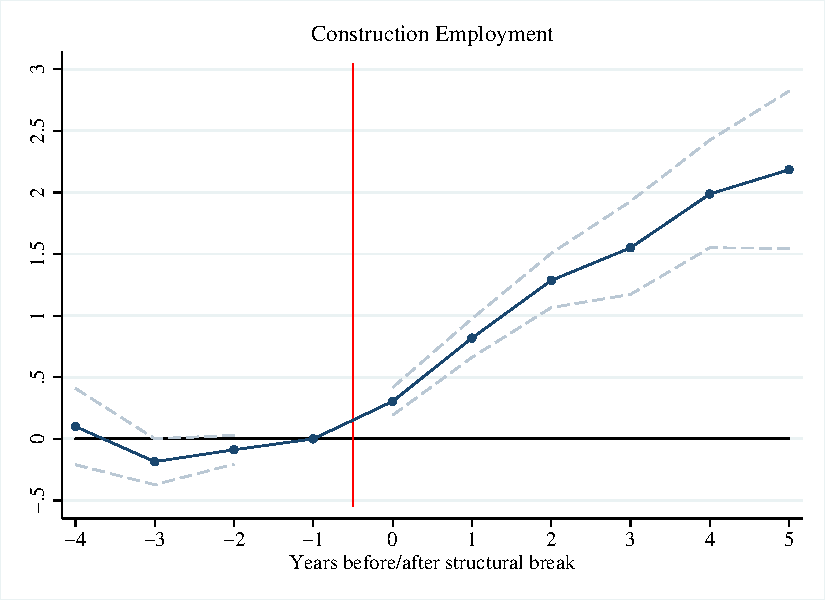
\includegraphics[scale=0.59]{output/cbp_evt_study_emp_cons_.pdf} \\
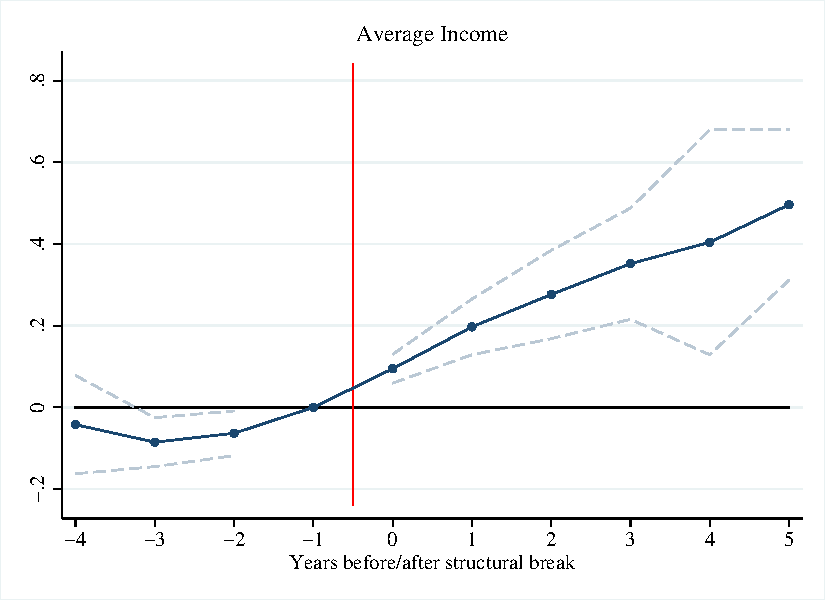
\includegraphics[scale=0.59]{output/cbp_evt_study_ave_ap_.pdf} \ \ \
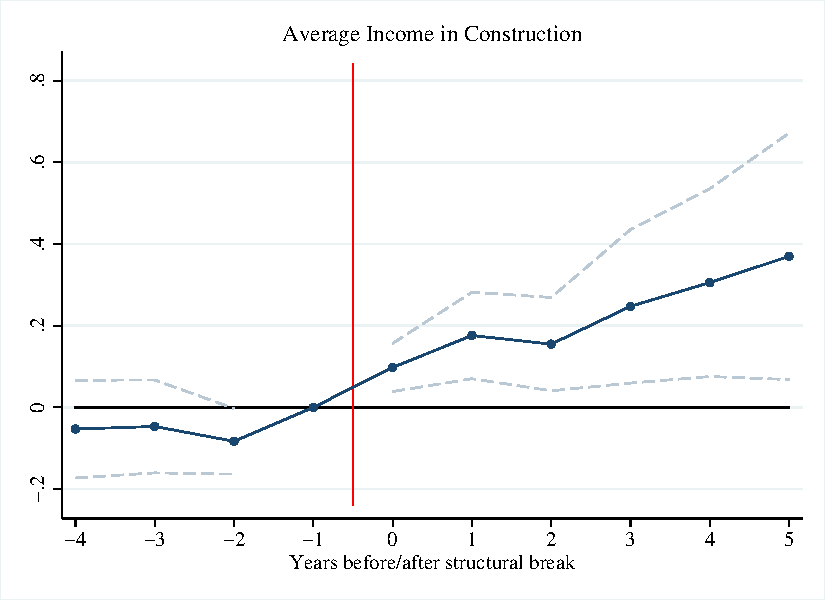
\includegraphics[scale=0.59]{output/cbp_evt_study_ave_ap_cons_.pdf} \\
\end{center}
\underline{Notes:} This figure reports estimates of event study regressions, which include indicator variables for each year before and after year of estimated structural break, which the indicator scaled by the magnitude of the structural break.  The event study regression specification includes year fixed effects and metropolitan area fixed effects and is weighted by the overall population in 1990.  The structural break is allowed to be anywhere between 1995Q1 and 2005Q1.  The employment and average income data come from the County Business Patterns (CBP) data, and the annual county-level data is matched to metropolitan areas using 2000 MSA definitions. The sample period in each metropolitan area is restricted to 6 years before and after estimated structural break (if available).  Standard errors are clustered by state.
\end{figure}





\clearpage 

\begin{figure}[!tp]
\begin{center}
Online Appendix Figure OA.5: Variation in Trends in Home Prices and Housing Permits Across Metropolitan Areas \\
\ \\
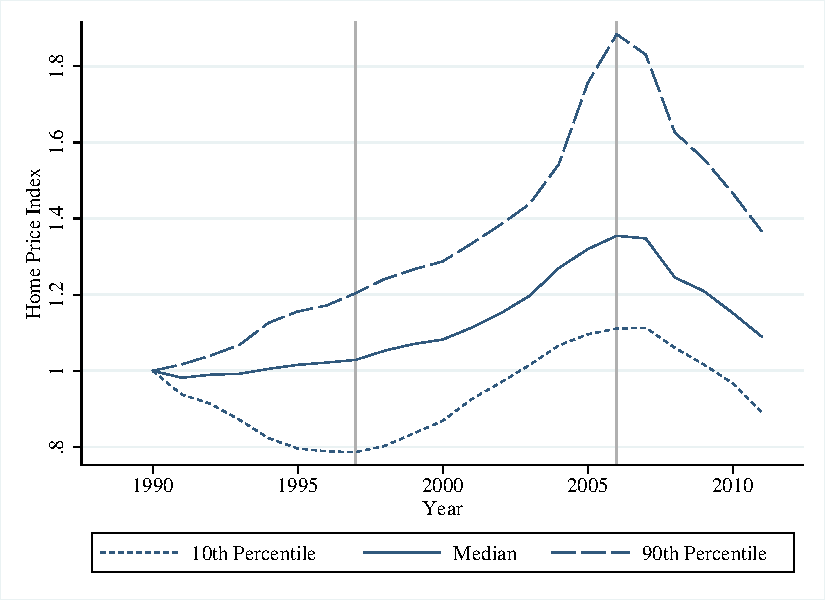
\includegraphics[scale=0.95]{output/fig_hpi_pctiles.pdf}
\ \\
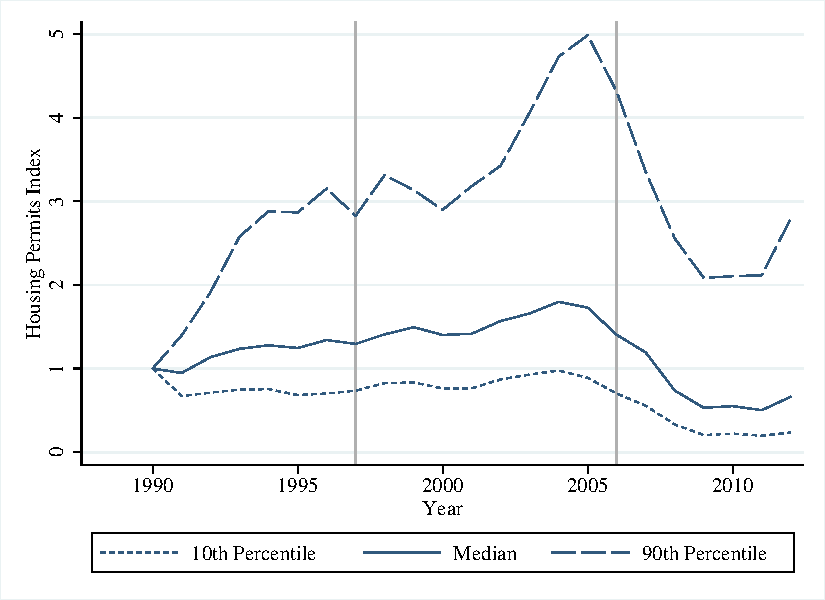
\includegraphics[scale=0.95]{output/fig_permits_pctiles.pdf}
\end{center}
\underline{Notes:} This figure reports trends in home prices and housing permits at the 10th percentile, median, and 90th percentile.  The home price data come from FHFA, and the housing permits data come from the Census.  Each metropolitan area series has been normalized by the year 1990 value before computing the percentiles each year.
\end{figure}



\begin{figure}[!tp]
\begin{center}
Online Appendix Figure OA.6: Trends in Educational Attainment for Men and Women, Age 18-29, 1980-2013 \\
\ \\
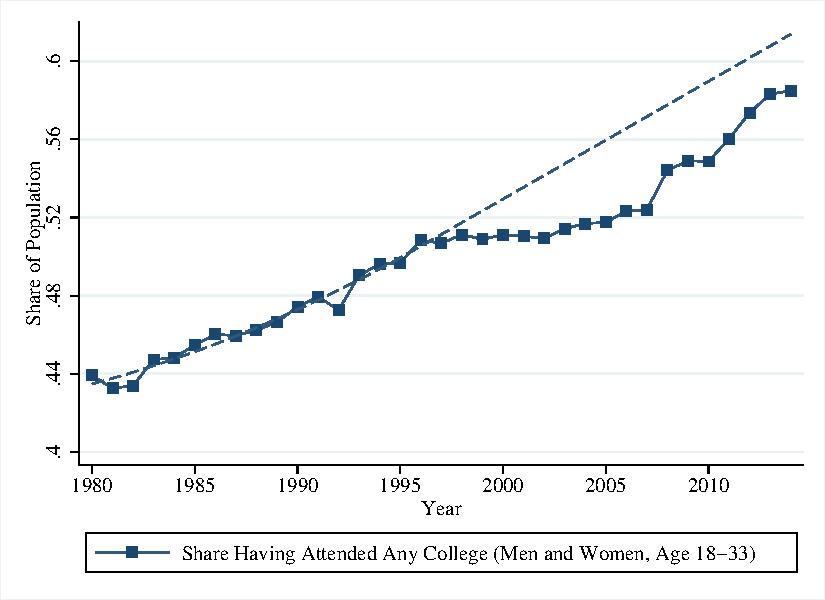
\includegraphics[scale=0.95]{output/educ_cps/fig_educ_all_18_29.pdf}
\end{center}
\underline{Notes:} This figure reports trends in the combined share of men and women (age 18-29) who have attended at least one year of college.  This series is constructed from the Current Population Survey.  The dashed line is the predicted college attendance rates based on a quadratic fit for 1980-1996 period.
\end{figure}

\clearpage


\begin{figure}[!tp]
\begin{center}
Online Appendix Figure OA.7: Trends in Cohort Effects in Educational Attainment for Individuals Born Between 1960 and 1990 \\
\ \\
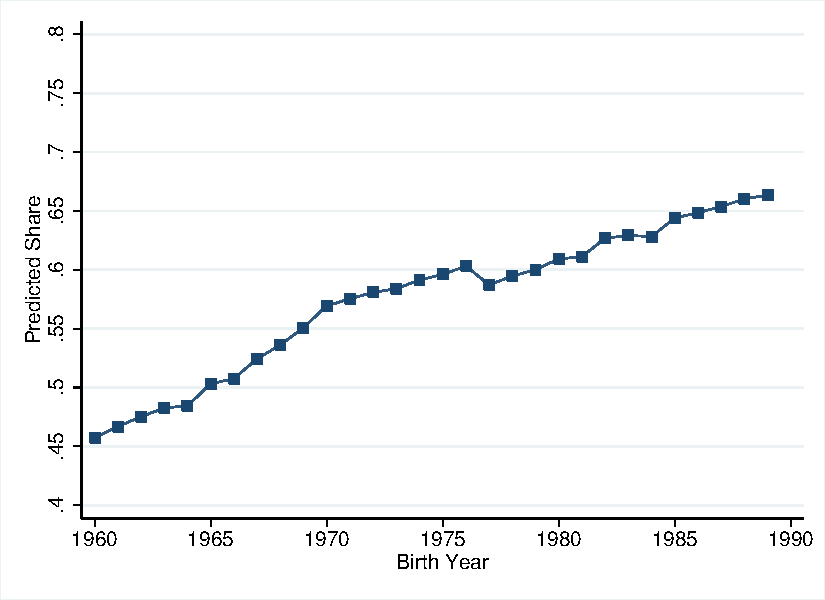
\includegraphics[scale=0.95]{output/educ_cps/cps_cohort_all.pdf} \\
\end{center}
\underline{Notes:} This figure reports estimated birth year (birth cohort) fixed effects in education for all men and women born between 1960 and 1990 (inclusive). The sample is all individuals between the ages of 25 and 54 in survey year pooling CPS data sets between 1994 and 2014.  The birth year fixed effects are recovered from an estimated model that regresses indicator for whether individual has attended any college on a fourth-degree polynomial in age, birth year fixed effects, and year fixed effects (excluding the first and last year). The figures reported fitted values at age 25 using CPS survey weights. The sample is restricted to native-born men and women.
\end{figure}



\clearpage

\begin{figure}[!tp]
\begin{center}
Online Appendix Figure OA.8: Seasonality in Housing Transactions \\
\ \\
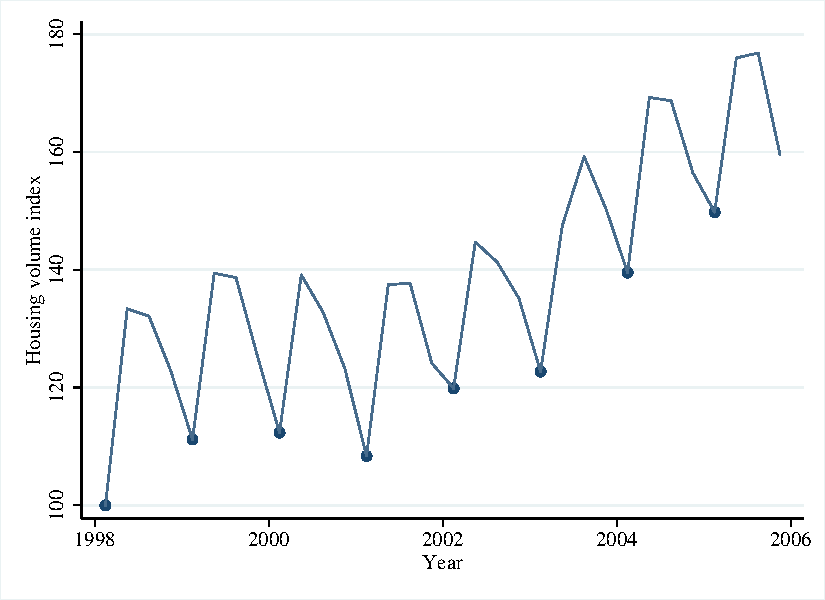
\includegraphics[scale=0.95]{output/fhfa/season_all.pdf} \\
\end{center}
\underline{Notes:} This figure reports quarterly housing transactions using DataQuick data from DeFusco et al. (2017). The solid circles indicate the first quarter for each year.
\end{figure}

\clearpage

\begin{figure}[!tp]
\begin{center}
Online Appendix Figure OA.9: Correlation Between Structural Break in Turnover and Prices \\
\ \\
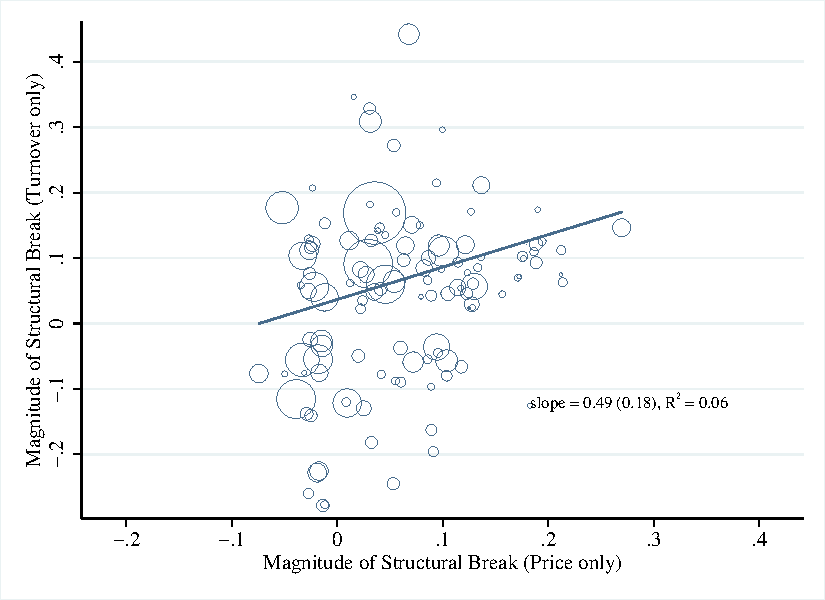
\includegraphics[scale=0.95]{output/fhfa/corr_turnover.pdf} \\
\end{center}
\underline{Notes:} This figure reports correlation between estimated magnitude of structural break in housing turnover (housing sales as a share of housing stock, from Zillow) and house prices (from FHFA data).
\end{figure}




\end{singlespace}
\end{document}
